% ----------------------------------------------------------
\chapter{FUNDAMENTAÇÃO TEÓRICA} \label{cap:Fundamentacao}
% ----------------------------------------------------------
\section{Sistemas Embarcados e Barramento CAN}

\begin{figure}[htbp]
    \centering
    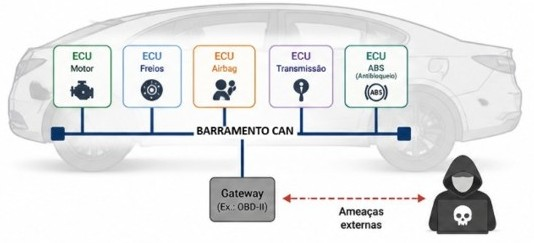
\includegraphics[width=0.6\textwidth]{images/CAN.jpeg}
    \caption{Entendimento do Barramento CAN}
    \label{fig:Protocolo_Can}
\end{figure}

O avanço tecnológico das últimas décadas modificou profundamente a arquitetura dos veículos modernos. Componentes que antes eram predominantemente mecânicos passaram a ser controlados por sistemas eletrônicos, formados por sensores, atuadores, unidades de controle e redes internas de comunicação. Nesse cenário, o veículo moderno pode ser compreendido como um sistema ciberfísico distribuído, no qual processos físicos, como frenagem, aceleração, direção, controle de estabilidade e gerenciamento do motor, são monitorados e controlados por componentes computacionais embarcados \cite{kukkala2018advanced}.

As unidades de controle eletrônico, conhecidas como \textit{Electronic Control Units} (ECUs), são responsáveis por executar funções específicas dentro do veículo. Cada ECU normalmente recebe sinais de sensores, processa essas informações e envia comandos para atuadores ou para outras ECUs \cite{navet2017automotive}. Como essas unidades não operam de forma isolada, a comunicação entre elas é fundamental para o funcionamento coordenado do sistema automotivo \cite{lin2012cyber}. Por exemplo, uma informação de velocidade pode ser utilizada simultaneamente pelo painel, pelo sistema de freios ABS, pelo controle de estabilidade e por sistemas de assistência ao condutor \cite{moller2019automotive}.

Essa integração trouxe ganhos expressivos de desempenho, conforto e segurança funcional. Entretanto, também aumentou a dependência dos veículos em relação à comunicação interna. Quanto maior o número de ECUs e de mensagens trocadas, maior tende a ser a complexidade da rede embarcada. Dessa forma, qualquer falha, atraso ou manipulação indevida nas mensagens pode afetar o comportamento de funções críticas do veículo \cite{bozdal2020evaluation}.

Entre os protocolos utilizados em redes internas automotivas, o CAN tornou-se um dos mais difundidos. O CAN foi projetado para permitir comunicação robusta, determinística e de baixo custo entre ECUs, sendo amplamente adotado na indústria automotiva devido à sua simplicidade, confiabilidade e capacidade de operar em ambientes sujeitos a ruídos eletromagnéticos \cite{specification1991bosch,navet2005trends}. O protocolo utiliza um modelo de comunicação baseado em broadcast, no qual as mensagens transmitidas no barramento podem ser recebidas por todos os nós conectados \cite{tindell1995calculating}.

Apesar de sua ampla adoção, o CAN foi desenvolvido originalmente em um contexto no qual a conectividade externa dos veículos era limitada. Por esse motivo, seu projeto priorizou requisitos como confiabilidade, arbitragem de mensagens e resposta em tempo real, deixando em segundo plano mecanismos de segurança da informação, como autenticação, confidencialidade e controle de acesso  \cite{lotto2024survey}. Como consequência, o protocolo não possui mecanismos nativos de criptografia nem autenticação de mensagens \cite{hanselmann2020canet}.

\subsection{Arquitetura de Comunicação em Redes Veiculares}

A arquitetura de comunicação de um veículo moderno é composta por diferentes redes internas, geralmente organizadas de acordo com os requisitos de cada domínio funcional \cite{douss2023state}. Sistemas relacionados ao trem de força, frenagem e controle de estabilidade demandam comunicação previsível e de baixa latência. Já sistemas de conforto, multimídia e diagnóstico podem tolerar atrasos maiores. Essa diversidade levou ao uso combinado de diferentes tecnologias, como CAN, CAN FD (\textit{Controller Area Network Flexible Data-Rate}), LIN (textit\{Local Interconnect Network}), FlexRay e Ethernet automotiva \cite{douss2023state,zeng2016vehicle}.

O barramento CAN permanece relevante porque oferece uma relação equilibrada entre custo, robustez e desempenho \cite{ben2020controller}. Essa característica decorre de sua arquitetura relativamente simples, baseada em comunicação serial por meio de um par diferencial de fios, o que reduz custos de implementação e manutenção \cite{specification1991bosch}. Além disso, o protocolo incorpora mecanismos eficientes de detecção e recuperação de erros, aumentando a confiabilidade da comunicação mesmo em ambientes sujeitos a interferências eletromagnéticas \cite{tindell1995calculating}. Do ponto de vista do desempenho, o CAN possibilita a transmissão de mensagens em tempo real e utiliza um mecanismo de arbitragem não destrutiva que garante prioridade às mensagens mais críticas, contribuindo para sua ampla adoção em sistemas automotivos e embarcados \cite{lin2022using}.

A arbitragem do CAN é não destrutiva \cite{sagstetter2013security}. Isso significa que, quando dois nós tentam transmitir ao mesmo tempo, o nó que transmite a mensagem de maior prioridade continua a transmissão, enquanto os demais interrompem e tentam novamente depois. Esse comportamento favorece aplicações de tempo real, pois permite que mensagens críticas tenham preferência sobre mensagens menos importantes \cite{lokman2019intrusion}.

No entanto, essa mesma característica pode ser explorada em ataques \cite{adly2023prevention}. Um nó malicioso que transmita continuamente mensagens de alta prioridade pode ocupar o barramento e impedir a transmissão de mensagens legítimas de menor prioridade. Além disso, como todos os nós recebem as mensagens, qualquer dispositivo conectado ao barramento pode observar o tráfego e, caso seja comprometido, pode tentar injetar mensagens falsas \cite{adly2023prevention}.

\subsection{Estrutura do Quadro CAN e Limitações de Segurança}

\begin{figure}[htbp]
    \centering
    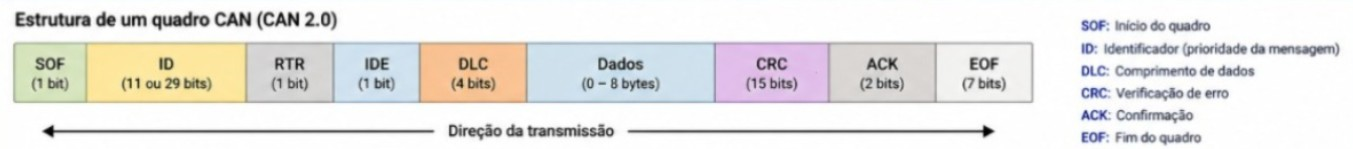
\includegraphics[width=1.0\textwidth]{images/CANstructure.jpg}
    \caption{Estrutura do CAN}
    \label{fig:Estrutura_Can}
\end{figure}

No CAN clássico, o campo de dados possui tamanho máximo de 8 bytes \cite{hartwich2012can} e essa limitação é importante quando se discute a aplicação de criptografia em sistemas veiculares, pois muitos algoritmos criptográficos foram projetados para operar com blocos de dados maiores. O AES, por exemplo, opera com blocos de 128 bits, ou seja, 16 bytes \cite{daemen2002design}. Assim, ao cifrar diretamente uma mensagem CAN clássica de 8 bytes com um algoritmo de bloco, pode ser necessário utilizar preenchimento ou reorganizar a forma de transmissão dos dados \cite{santos2025aplicabilidade}.

A estrutura básica de um quadro CAN inclui campos como início de quadro, identificador, campo de controle, dados, CRC, confirmação e fim de quadro \cite{de2018transmissao}. Embora o CRC contribua para a detecção de erros acidentais de transmissão, ele não oferece proteção criptográfica. Um atacante que consiga injetar mensagens pode recalcular o CRC e produzir um quadro aparentemente válido. Por isso, mecanismos de integridade não criptográficos não devem ser confundidos com mecanismos de autenticação \cite{avatefipour2018state}.

A ausência de autenticação é um dos principais problemas do CAN. Como o protocolo não verifica se uma mensagem foi realmente emitida por uma ECU legítima, qualquer nó com acesso ao barramento pode transmitir mensagens usando identificadores válidos. Isso torna possíveis ataques de falsificação, injeção e repetição de mensagens. A ausência de confidencialidade também permite que o tráfego seja observado por dispositivos conectados, facilitando a engenharia reversa de identificadores e padrões de comunicação \cite{chandwani2020cybersecurity}.

\subsection{CAN Clássico e CAN FD}

\begin{figure}[htbp]
    \centering
    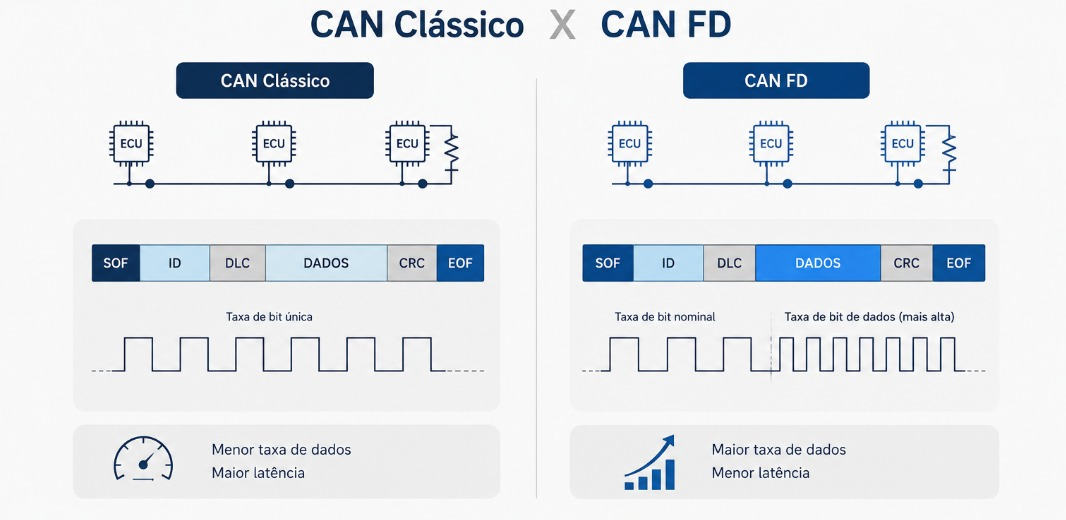
\includegraphics[width=1.0\textwidth]{images/comparacaoCAN.jpeg}
    \caption{Comparação de CAN Clássico com CAN FD}
    \label{fig:Comparação_Can}
\end{figure}

O CAN clássico apresenta limitações relevantes para aplicações modernas, especialmente em relação à largura de banda e ao tamanho do campo de dados. Para superar parte dessas restrições, foi desenvolvido o CAN FD, que permite maior carga útil por quadro e taxas de transmissão mais altas durante a fase de dados. Enquanto o CAN clássico transporta até 8 bytes de dados, o CAN FD pode transportar até 64 bytes \cite{xiao2020session}.

Nesse contexto, a ampliação da carga útil proporcionada pelo CAN FD possui impacto direto na implementação de mecanismos criptográficos. Em um quadro CAN clássico, inserir um código de autenticação de mensagem ou um valor criptográfico adicional pode consumir parte significativa da carga útil disponível. Já no CAN FD, há mais espaço para incluir campos de autenticação, contadores, nonces ou etiquetas criptográficas. Por essa razão, propostas recentes de segurança para redes veiculares frequentemente consideram o CAN FD como um ambiente mais flexível para aplicação de criptografia e autenticação \cite{nurnberger2016vatican}.

Apesar disso, muitos veículos ainda utilizam CAN clássico em diferentes domínios internos. Assim, a análise de algoritmos criptográficos para mensagens curtas continua relevante. Um algoritmo eficiente em grandes blocos de dados pode não apresentar o mesmo comportamento quando aplicado a mensagens pequenas e frequentes. Esse ponto é central para este trabalho, pois a comparação entre tipos de criptografia deve considerar não apenas a segurança teórica, mas também a adequação ao tamanho real das mensagens do barramento \cite{nowdehi2017vehicle}.

\subsection{Restrições de Tempo Real em Sistemas Automotivos}

Sistemas automotivos embarcados frequentemente operam sob restrições de tempo real, nas quais a corretude do sistema depende não apenas da execução lógica das tarefas, mas também do cumprimento de prazos temporais previamente definidos \cite{buttazzo1997hard}. Em sistemas de tempo real, uma resposta produzida após o instante limite estabelecido pode ser considerada incorreta, mesmo que o resultado computacional esteja correto \cite{kopetz1997real}. Em aplicações automotivas como controle de motor, frenagem eletrônica e controle de estabilidade, atrasos excessivos podem comprometer o funcionamento adequado do sistema e afetar requisitos de segurança operacional \cite{nolte2017timing}. Por esse motivo, qualquer mecanismo adicional inserido no caminho de comunicação, incluindo técnicas criptográficas, precisa ser cuidadosamente avaliado quanto ao impacto que provoca na latência e no desempenho geral da rede \cite{bruton2014securing}.

A latência total percebida por uma mensagem protegida não depende apenas do tempo de transmissão no barramento. Ela também inclui o tempo necessário para processar a mensagem antes da transmissão e, eventualmente, após a recepção. Quando se adiciona criptografia, há um custo computacional associado à cifragem, decifragem, geração de etiquetas de autenticação ou verificação de integridade \cite{schmandt2017mini}.

Em sistemas de tempo real, mesmo atrasos pequenos podem se tornar relevantes quando acumulados em grande volume de mensagens. Uma ECU pode transmitir mensagens em intervalos de poucos milissegundos, e um veículo pode possuir dezenas de unidades trocando informações continuamente. Assim, a comparação entre algoritmos criptográficos deve considerar o atraso por operação, a variabilidade e o impacto acumulado ao longo do tempo (Fig.~\ref{fig:Criptografia}) \cite{ravi2020authentication}. 

\section{Criptografia e Tipos de Algoritmos Usados}

\begin{figure}[htbp]
    \centering
    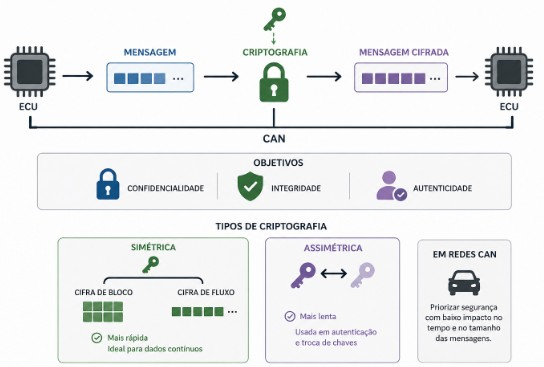
\includegraphics[width=1.0\textwidth]{images/Criptografia.jpg}
    \caption{Entendimento da Criptografia em Barramento CAN}
    \label{fig:Criptografia}
\end{figure}

A criptografia é um mecanismo fundamental para a proteção de dados, sendo responsável por garantir propriedades como confidencialidade, integridade e autenticidade das informações transmitidas \cite{menezes2018handbook}. Em sistemas embarcados e redes veiculares, sua aplicação torna-se especialmente relevante devido à ausência de mecanismos nativos de segurança em protocolos como o CAN \cite{ribeiro2024decodificando}. Nesse contexto, a utilização de mecanismos criptográficos busca mitigar vulnerabilidades relacionadas à autenticidade, integridade e confidencialidade das mensagens transmitidas.

Considerando as restrições temporais discutidas anteriormente, a utilização de criptografia em redes automotivas deve ser analisada de forma diferente daquela aplicada em sistemas computacionais convencionais. Por esse motivo, a criptografia aplicada ao barramento CAN não deve ser avaliada apenas pelo nível de segurança oferecido, mas também pelo impacto que produz sobre o tempo de processamento, o tamanho das mensagens e o consumo de recursos computacionais \cite{diao2011resource}.

Além disso, a proteção de mensagens em barramentos automotivos não se limita à confidencialidade. Em muitos casos, impedir que uma mensagem seja lida pode ser menos importante do que garantir que ela não foi modificada e que foi enviada por uma ECU legítima. Assim, propriedades como integridade e autenticação assumem papel central em redes CAN, uma vez que o protocolo utiliza comunicação em broadcast e não possui mecanismos nativos para verificar a identidade do nó transmissor. Como consequência, dispositivos maliciosos ou comprometidos podem injetar mensagens fraudulentas no barramento, dificultando a distinção entre mensagens legítimas e mensagens adulteradas \cite{lotto2024survey}. Essa característica torna relevante a análise de algoritmos e mecanismos capazes de proteger as mensagens sem comprometer a operação contínua do sistema \cite{basavaraj2022towards}.

Os algoritmos criptográficos podem ser classificados em duas categorias principais: criptografia simétrica e criptografia assimétrica. No contexto da criptografia simétrica, distinguem-se ainda duas abordagens estruturais: cifras de bloco e cifras de fluxo \cite{forouzan2007cryptography}. Essas categorias apresentam características distintas em termos de desempenho, custo computacional e aplicabilidade em ambientes com restrições de recursos \cite{dudhat2024comparative}.

A distinção entre essas categorias é importante, porque cada tipo de algoritmo tende a se comportar de maneira diferente quando aplicado a mensagens curtas. Enquanto algoritmos simétricos normalmente apresentam melhor desempenho para cifragem contínua de dados, algoritmos assimétricos possuem maior custo computacional e são mais adequados para operações pontuais, como autenticação inicial ou troca de chaves \cite{meng2020lightweight}. Dentro dos algoritmos simétricos, cifras de bloco e cifras de fluxo também apresentam diferenças relevantes, principalmente em relação ao tamanho mínimo de processamento e à necessidade de preenchimento dos dados \cite{sharif2010performance}.

\subsection{Criptografia Simétrica}

\begin{figure}[htbp]
    \centering
    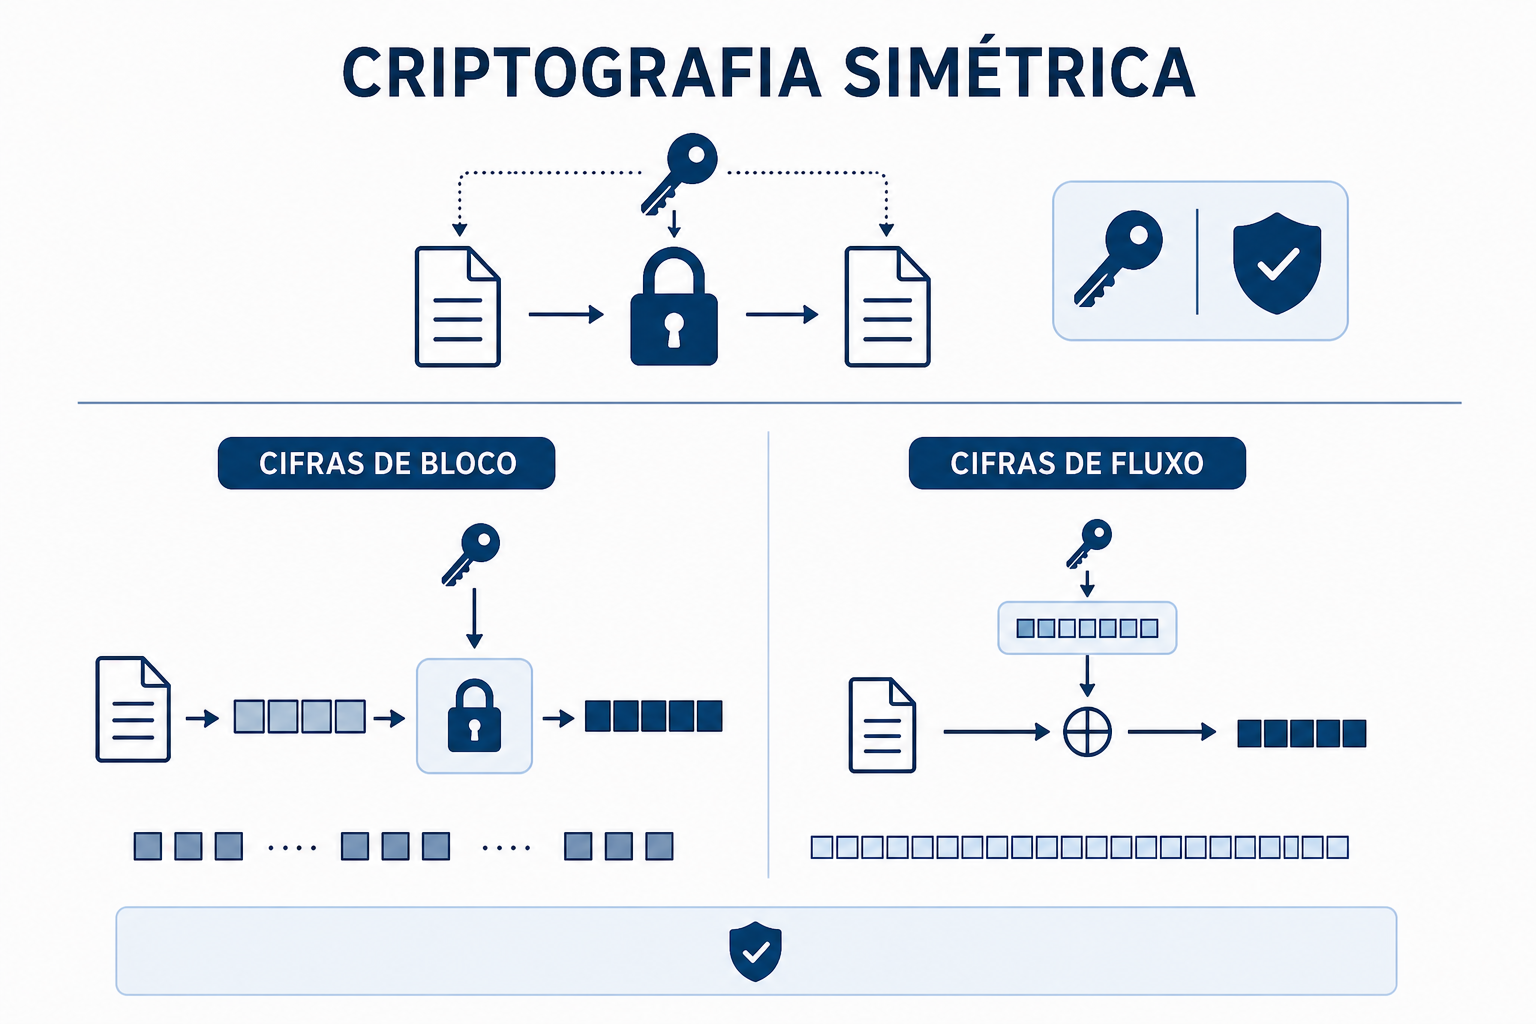
\includegraphics[width=1.0\textwidth]{images/simetrica.jpg}
    \caption{Entendimento da Criptografia Simétrica}
    \label{fig:Criptografia-Simetrica}
\end{figure}

A criptografia simétrica utiliza uma única chave secreta compartilhada para cifragem e decifragem, sendo amplamente empregada em aplicações que exigem baixo tempo de processamento e alta eficiência computacional \cite{paar2010understanding}. Esses algoritmos apresentam custo computacional significativamente inferior aos assimétricos, sendo adequados para processamento contínuo de dados em sistemas embarcados \cite{kaps2006cryptography}.

No contexto de redes CAN, a criptografia simétrica apresenta maior viabilidade prática para proteção direta de mensagens, pois permite tempos de execução menores e menor consumo de recursos. Como as mensagens podem ser transmitidas em alta frequência, especialmente em sistemas de controle veicular, o uso de algoritmos com baixo custo por operação é essencial para evitar aumento significativo da latência \cite{mundhenk2015lightweight}. Essa característica torna os algoritmos simétricos candidatos naturais para avaliações de desempenho em ambientes embarcados \cite{thakor2021lightweight}.

Outro ponto relevante é que a criptografia simétrica pode ser combinada com mecanismos de autenticação de mensagens, como códigos de autenticação de mensagem (\textit{Message Authentication Codes} -- MACs). Nesse caso, a chave compartilhada não é utilizada apenas para cifrar dados, mas também para verificar a integridade e a origem da mensagem \cite{vacca2017computer}. Essa abordagem é especialmente importante em redes CAN, nas quais ataques de falsificação e repetição de mensagens podem ocorrer devido à ausência de autenticação nativa \cite{gallagher2025enhancing}.

No contexto deste trabalho, a criptografia simétrica é subdividida em cifras de bloco e cifras de fluxo \cite{yung2010applied}.

Cifras de bloco operam sobre unidades de tamanho fixo. O \textit{Advanced Encryption Standard} (AES) processa blocos de 128 bits (16 bytes) \cite{dworkin2001recommendation,primitives2003advanced}.

\begin{figure}[htbp]
    \centering
    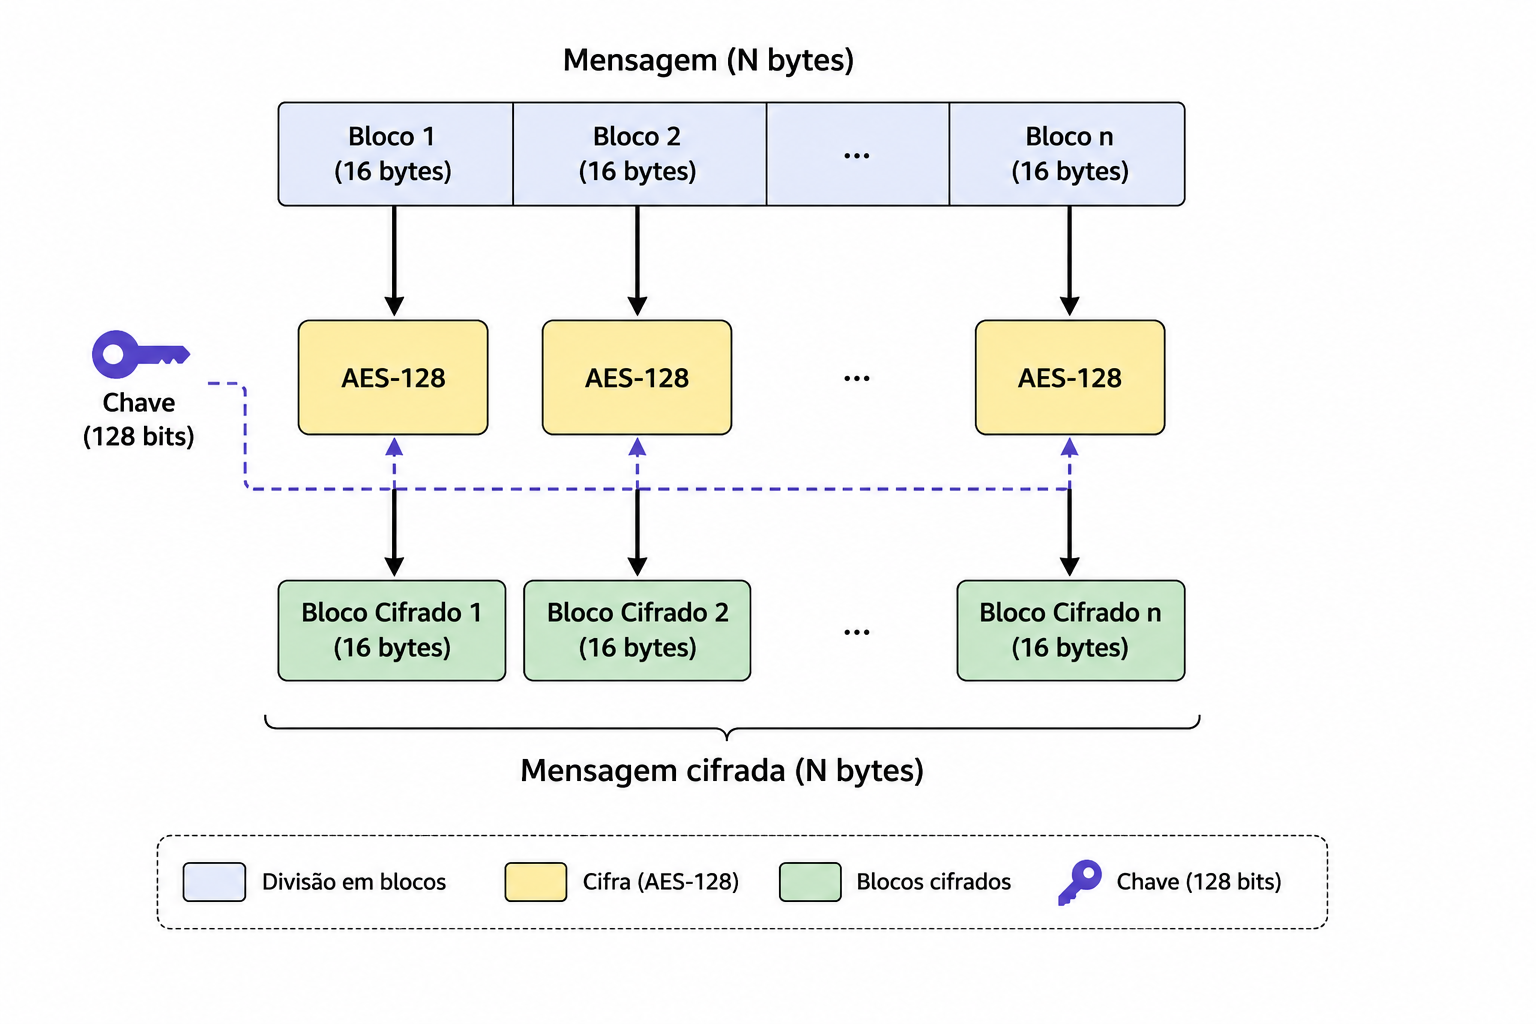
\includegraphics[width=1.0\textwidth]{images/cifrabloco.jpg}
    \caption{Diagrama de uma Cifra de Bloco}
    \label{fig:Cifra-Bloco}
\end{figure}

No barramento CAN clássico, cujo campo de dados possui até 8 bytes, há incompatibilidade estrutural. Nesse contexto, o overhead corresponde ao aumento relativo do tamanho da mensagem após a cifragem:

\begin{equation}
\text{Overhead} = \frac{T_{final} - T_{original}}{T_{original}}
\end{equation}

Em um exemplo hipotético de modo que exige preenchimento para completar um bloco de 16 bytes, uma entrada de 8 bytes pode ocupar 16 bytes:

\begin{equation}
\text{Overhead} = \frac{16 - 8}{8} = 1 \quad (100\%)
\end{equation}

Esse aumento hipotético não se aplica automaticamente ao AES-128-CTR, modo utilizado neste trabalho, pois o CTR não exige preenchimento e preserva o comprimento do texto cifrado. Ainda assim, parâmetros como nonce e contador precisam ser gerenciados e podem exigir informações adicionais no protocolo. Quando ocorre expansão do conteúdo transmitido, ela implica crescimento do volume de dados processados e pode impactar tanto o tempo de processamento quanto a ocupação do barramento \cite{chen2019performance}.

O CAN clássico possui uma carga útil reduzida e quando um algoritmo exige blocos maiores do que o tamanho original da mensagem, parte da capacidade disponível passa a ser utilizada apenas para adequação estrutural da cifra, e não necessariamente para transmissão de informação útil. Em sistemas nos quais a ocupação do barramento já é elevada, esse aumento pode reduzir a margem disponível para novas mensagens ou para mecanismos adicionais de segurança \cite{fernandez2024cybersecurity}.

O custo computacional pode ser modelado como:

\begin{equation}
T_{proc} = T_{fixo} + n_{blocos} \cdot T_{bloco}
\end{equation}

\noindent onde $T_{fixo}$ representa o custo de inicialização do contexto criptográfico \cite{tanenbaum2016structured}. Evidenciando que o tempo de processamento de uma cifra de bloco não depende apenas da quantidade total de bytes, mas também da quantidade de blocos processados. Para mensagens muito pequenas, como as mensagens do CAN clássico, o custo fixo pode se tornar proporcionalmente mais relevante do que o custo associado aos dados propriamente ditos. Dessa forma, mesmo que o AES seja altamente eficiente em muitos ambientes, sua aplicação em mensagens de 8 bytes exige análise cuidadosa, principalmente quando não há aceleração por hardware disponível \cite{dhanda2025aes}.

Embora o AES seja frequentemente tratado como um algoritmo único, sua aplicação prática depende do modo de operação utilizado, que determina como os blocos de dados são processados e encadeados ao longo da mensagem. Entre os modos mais conhecidos estão o Electronic Codebook (ECB), o Cipher Block Chaining (CBC), o Counter Mode (CTR) e o Galois/Counter Mode (GCM) \cite{dworkin2001recommendation}.

O modo ECB é desaconselhado em aplicações reais, pois blocos de texto claro iguais produzem blocos cifrados iguais, revelando padrões da mensagem original \cite{bellare2005introduction}. O modo CBC reduz esse problema ao introduzir dependência entre blocos consecutivos, mas essa dependência pode dificultar paralelização e aumentar o custo em determinados cenários \cite{ferguson2011cryptography}. Já o modo CTR transforma a cifra de bloco em uma estrutura semelhante a uma cifra de fluxo, permitindo maior paralelismo e evitando parte das limitações associadas ao encadeamento sequencial \cite{lipmaa2000ctr}.

O modo GCM, por sua vez, é amplamente utilizado por combinar confidencialidade e autenticação em uma única construção \cite{mcgrew2004galois}. EEssa característica é particularmente relevante para redes veiculares, uma vez que o protocolo CAN não possui mecanismos nativos para verificar a origem das mensagens transmitidas, tornando possível a injeção de mensagens fraudulentas por dispositivos comprometidos ou não autorizados \cite{lotto2024survey}. No entanto, modos autenticados normalmente exigem a transmissão ou armazenamento de informações adicionais, como vetores de inicialização, contadores ou etiquetas de autenticação. Em mensagens CAN clássicas, nas quais o campo de dados é limitado a 8 bytes, esse overhead deve ser cuidadosamente considerado \cite{de2023security}.

Dessa forma, ao avaliar o AES, não basta considerar apenas o algoritmo em si, sendo necessário observar também o modo de operação utilizado, pois ele influencia diretamente no tempo de processamento, no volume de dados adicional e o nível de proteção obtido \cite{fazzat2020comparative}.

O desempenho do AES pode variar significativamente conforme o ambiente de execução, uma vez que processadores modernos frequentemente disponibilizam instruções específicas de aceleração criptográfica, como o AES-NI, capazes de reduzir consideravelmente o tempo de cifragem e tornar o algoritmo mais eficiente \cite{gueron2010intel}. Entretanto, em muitos sistemas embarcados, especialmente aqueles baseados em microcontroladores de menor custo, esse tipo de aceleração pode não estar disponível \cite{eisenbarth2007survey}.

Na ausência de aceleração por hardware, o AES depende exclusivamente da implementação em software, que aumenta o tempo de execução e o consumo de CPU \cite{aziz2007memory}. Esse aspecto é relevante para o presente trabalho, pois a comparação entre algoritmos deve considerar não apenas a segurança teórica, mas também as condições reais de execução. Um algoritmo amplamente eficiente em servidores ou computadores pessoais pode apresentar comportamento diferente quando executado em um ambiente embarcado restrito \cite{beaulieu2015simon}.

Assim, a análise de desempenho do AES deve ser interpretada de forma contextualizada. Caso o ambiente possua aceleração por hardware, o AES tende a apresentar desempenho elevado e previsível. Caso contrário, cifras de fluxo como o ChaCha20 podem se tornar mais competitivas, especialmente em aplicações que processam mensagens curtas e frequentes \cite{nir2018chacha20}.

Cifras de fluxo operam sobre dados de forma contínua, processando pequenas unidades de informação à medida que são transmitidas, em vez de dividir a mensagem em blocos de tamanho fixo. Nesse modelo, uma sequência pseudoaleatória de \textit{bits}, denominada fluxo de chave (\textit{keystream}), é combinada com os dados originais para produzir o texto cifrado. Essa abordagem é particularmente adequada para aplicações que exigem baixa latência ou transmissão contínua de dados, como sistemas embarcados e comunicações em tempo real \cite{menezes2018handbook}. Um exemplo clássico de cifra de fluxo foi o \textit{Rivest Cipher 4} (RC4), amplamente utilizado em protocolos de comunicação durante muitos anos, embora atualmente seja considerado inseguro devido a vulnerabilidades descobertas ao longo do tempo \cite{alfardan2013security}. Entre as alternativas modernas, destaca-se o algoritmo ChaCha20, que apresenta elevado desempenho em software e comportamento aproximadamente proporcional ao volume de dados processados \cite{bernstein2008chacha,manifavas2016survey}.

Seu custo computacional pode ser representado por:

\begin{equation}
T_{proc} = T_{fixo} + D \cdot C_{byte}
\end{equation}

onde $C_{byte}$ representa o custo médio por \textit{byte} processado.

Essa estrutura elimina a necessidade de padding e evita overhead estrutural, sendo particularmente adequada para mensagens curtas e frequentes \cite{arciszewski2020xchacha}.

A ausência de padding é uma característica importante no contexto do CAN clássico. Como a mensagem possui tamanho reduzido, qualquer \textit{byte} adicional representa uma parcela significativa da carga útil disponível. Cifras de fluxo, por operarem diretamente sobre a sequência de \textit{bytes} da mensagem, permitem que o tamanho cifrado acompanhe mais diretamente o tamanho original dos dados. Isso reduz o desperdício estrutural e facilita a aplicação do modelo de custo por \textit{byte} \cite{indira2020light}.

\subsection{ChaCha20 e Desempenho em Software}

\begin{figure}[htbp]
    \centering
    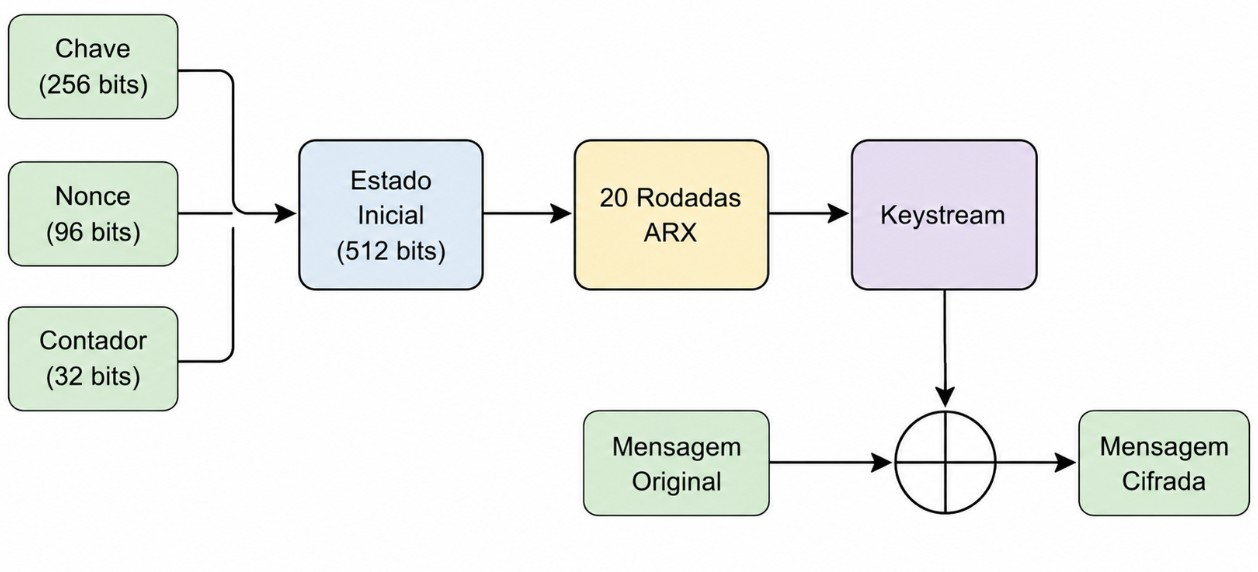
\includegraphics[width=1.0\textwidth]{images/chacha20.jpg}
    \caption{Fluxograma do ChaCha20}
    \label{fig:ChaCha20}
\end{figure}

O funcionamento do ChaCha20 baseia-se na geração de um fluxo pseudoaleatório de bits (\textit{keystream}), produzido a partir de uma chave secreta, um contador e um valor único denominado nonce. Inicialmente, esses elementos são organizados em uma matriz interna de 512 \textit{bits}. Em seguida, são aplicadas sucessivas rodadas de operações ARX (\textit{Addition}, \textit{Rotation} and \textit{XOR}), que promovem difusão e confusão dos dados. Ao final do processamento, o bloco gerado é combinado com a mensagem original por meio da operação XOR, produzindo o texto cifrado \cite{bernstein2008chacha,dinu2017efficient}. Essas operações são eficientes em diferentes arquiteturas de processadores e não dependem de instruções especializadas para alcançar bom desempenho \cite{nir2018chacha20}.

O ChaCha20 apresenta características particularmente adequadas para mensagens CAN, pois, por ser uma cifra de fluxo, não exige o particionamento dos dados em blocos de tamanho fixo nem a utilização de mecanismos de preenchimento (\textit{padding}) para completar blocos incompletos. Dessa forma, o custo computacional tende a acompanhar de maneira mais direta o volume de dados processado, o que facilita a estimativa da latência por mensagem e a comparação com outros algoritmos \cite{manifavas2016survey}.

\subsection{Cifras de Fluxo e Cuidados de Segurança}

Apesar de suas vantagens de desempenho, cifras de fluxo exigem cuidados específicos de implementação. Um dos principais requisitos é evitar a reutilização do mesmo fluxo de chave para mensagens diferentes. Caso o mesmo par chave/nonce seja reutilizado, informações sobre os textos originais podem ser inferidas, comprometendo a segurança da comunicação \cite{bernstein2005poly1305}.

Em sistemas veiculares, esse cuidado é particularmente relevante porque muitas mensagens CAN são transmitidas ciclicamente com identificadores fixos e conteúdo previsível. Como consequência, a reutilização de pares chave/\textit{nonce} pode resultar na repetição do \textit{keystream} utilizado pela cifra, permitindo que informações sobre as mensagens originais sejam inferidas por um atacante \cite{bernstein2005poly1305,lin2012cyber}.

Portanto, embora o ChaCha20 apresente vantagens claras de desempenho, sua aplicação prática deve considerar não apenas o tempo de cifragem, mas também o gerenciamento seguro dos parâmetros associados à cifra. Essa observação reforça que a escolha do algoritmo não deve ser feita apenas com base no desempenho bruto, mas considerando o conjunto completo de requisitos de segurança \cite{meng2020lightweight}.

\subsection{Criptografia Assimétrica}

\begin{figure}[htbp]
    \centering
    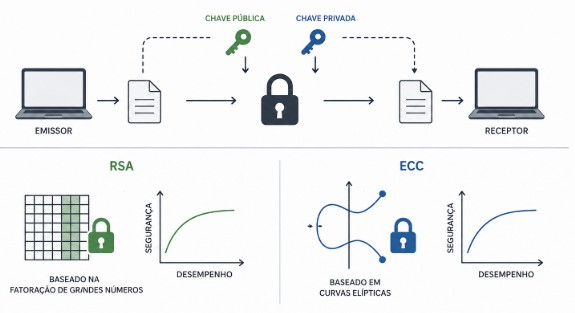
\includegraphics[width=1.0\textwidth]{images/assimetrica.jpg}
    \caption{Entendimento da Criptografia Assimétrica}
    \label{fig:Criptografia-Assimetrica}
\end{figure}

Algoritmos assimétricos utilizam pares de chaves e baseiam-se em problemas matemáticos complexos \cite{diffie2022new,rivest1978method,miller1985use}. Seu custo computacional é significativamente superior, frequentemente na ordem de milissegundos por operação em CPUs de propósito geral, em contraste com algoritmos simétricos que operam na ordem de microssegundos \cite{micali1992fair}. Dessa forma, sua utilização em sistemas embarcados é restrita a operações pontuais, como autenticação e troca de chaves \cite{gura2004comparing}.

A criptografia assimétrica resolve um problema que a criptografia simétrica não resolve sozinha: a distribuição segura de chaves. Em um sistema com diversas ECUs, o uso de uma chave secreta compartilhada exige que essa chave seja armazenada, protegida e atualizada ao longo do ciclo de vida do veículo. Algoritmos assimétricos podem auxiliar nesse processo, permitindo o estabelecimento de chaves de sessão ou a autenticação inicial entre entidades \cite{mundhenk2017security}.

No entanto, utilizar algoritmos assimétricos diretamente em cada mensagem CAN não é uma abordagem adequada para a maioria dos cenários. O tamanho das chaves, o tempo de processamento e o volume de dados adicionais tornam essa aplicação incompatível com a carga útil limitada e com os requisitos temporais do barramento \cite{tian2020secure}. Assim, a criptografia assimétrica tende a ser mais adequada em uma arquitetura híbrida, na qual é utilizada em momentos específicos, enquanto algoritmos simétricos protegem a comunicação contínua \cite{muter2010structured}.

Entre os mecanismos assimétricos considerados neste trabalho, destaca-se o Rivest--Shamir--Adleman (RSA), cuja segurança está relacionada à dificuldade de fatoração de grandes números inteiros \cite{boneh1999twenty}. Outra abordagem é a criptografia de curvas elípticas, denominada \textit{Elliptic Curve Cryptography} (ECC), que reúne técnicas baseadas em operações matemáticas sobre pontos de curvas elípticas e no problema do logaritmo discreto nesse contexto \cite{miller1985use,galbraith2012mathematics}. A ECC não corresponde, isoladamente, a um algoritmo de cifragem de dados, mas oferece operações utilizadas, por exemplo, no estabelecimento de segredos compartilhados e em assinaturas digitais.

Para representar uma aplicação de cifragem baseada em curvas elípticas, este trabalho utiliza uma construção híbrida inspirada no \textit{Elliptic Curve Integrated Encryption Scheme} (ECIES), identificada como ECIES-P256 \cite{ieee1363a2004}. Nessa abordagem, a criptografia de curvas elípticas participa do estabelecimento de um segredo por meio do \textit{Elliptic Curve Diffie--Hellman} (ECDH), empregando a curva P-256 \cite{miller1985use}. A partir desse segredo, obtém-se material de chave para uma operação simétrica responsável pela cifragem efetiva dos dados. Assim, o ECIES combina técnicas assimétricas e simétricas em vez de cifrar a mensagem diretamente por meio de uma operação de curva elíptica \cite{ieee1363a2004}.

A escolha do ECIES-P256 permite observar o custo computacional de uma construção híbrida que utiliza ECC em um cenário de mensagens curtas. Sua inclusão não pressupõe que a etapa assimétrica deva ser repetida para cada quadro CAN em uma implementação automotiva real: o estabelecimento de chaves pode ocorrer em fases específicas da comunicação, enquanto a proteção contínua dos dados pode ser realizada por mecanismos simétricos \cite{mundhenk2017security}. Por isso, os tempos associados ao ECIES-P256 devem ser interpretados de acordo com as etapas efetivamente executadas e temporizadas pelo programa, sem equipará-los automaticamente aos tempos de cifragem isolada de AES-128-CTR e ChaCha20.

A comparação entre RSA-2048-OAEP e ECIES-P256 também requer cautela. O primeiro é um mecanismo de cifragem assimétrica com preenchimento OAEP \cite{rfc8017}; o segundo constitui uma construção híbrida \cite{ieee1363a2004}. Embora ambos possam ser estudados no contexto de proteção e estabelecimento de material criptográfico, não realizam operações idênticas. Desse modo, a avaliação apresentada neste trabalho busca caracterizar seus custos computacionais e suas possíveis funções em uma arquitetura de segurança, e não estabelecer uma classificação universal de desempenho entre mecanismos com finalidades distintas.

Apesar de sua importância para mecanismos de segurança, a criptografia assimétrica apresenta limitações significativas em sistemas embarcados de tempo real. O elevado custo computacional dessas operações pode introduzir atrasos incompatíveis com os requisitos temporais de aplicações críticas \cite{gaubatz2004public}.

Além disso, operações como geração de chaves e assinatura digital demandam maior uso de memória e processamento, o que pode comprometer a execução de outras tarefas no sistema \cite{qazi2021security}. Por esse motivo, sua aplicação em redes CAN é geralmente restrita a fases de inicialização, como estabelecimento de chaves, sendo evitada durante a transmissão contínua de mensagens \cite{luo2021can}.

Essa limitação reforça a necessidade de utilização de algoritmos simétricos ou mecanismos híbridos, nos quais a criptografia assimétrica é utilizada apenas para distribuição segura de chaves \cite{hammi2018bubbles}.

O desenvolvimento de algoritmos de criptografia leve tem ganhado destaque nos últimos anos, especialmente em aplicações relacionadas à IoT e sistemas embarcados automotivos. Esses algoritmos são projetados para operar com baixo consumo de energia, memória reduzida e menor complexidade computacional, mantendo níveis adequados de segurança \cite{beaulieu2015simon}.

Entre os algoritmos mais estudados nesse contexto destacam-se soluções como PRESENT, SPECK, SIMON e, mais recentemente, o ASCON, selecionado como padrão pelo NIST para criptografia leve \cite{bogdanov2007present,biryukov2014differential,dobraunig2021ascon}. Esses algoritmos apresentam estruturas simplificadas quando comparados a soluções tradicionais como o AES, o que pode resultar em melhor desempenho em dispositivos com recursos limitados \cite{sadkhan2018survey}.

No contexto do barramento CAN, a utilização de criptografia leve representa uma alternativa promissora, especialmente devido ao tamanho reduzido das mensagens e às restrições de tempo real \cite{sagstetter2013security}. No entanto, sua adoção deve considerar cuidadosamente o nível de segurança oferecido, uma vez que simplificações estruturais podem impactar a resistência a ataques criptográficos \cite{manifavas2013lightweight}.

A criptografia leve também deve ser analisada sob o ponto de vista da padronização e da maturidade das implementações. Algoritmos amplamente padronizados e analisados pela comunidade tendem a oferecer maior confiança para aplicações críticas \cite{kaur2025survey}. Em sistemas automotivos, nos quais falhas podem afetar segurança funcional, a adoção de um algoritmo não depende apenas de bom desempenho, mas também de confiança, documentação, interoperabilidade e resistência a ataques conhecidos \cite{ponsard2016goal}.

Dessa forma, embora algoritmos leves sejam relevantes, sua comparação com algoritmos tradicionais deve ser feita com cautela, buscando não é apenas identificar o algoritmo mais rápido, mas compreender qual solução apresenta melhor equilíbrio entre desempenho, segurança e viabilidade de implementação em mensagens de barramento CAN \cite{iqbal2025design}.

\subsection{Exemplo de Aplicação dos Algoritmos em Mensagens CAN}

Para ilustrar a aplicação prática dos algoritmos estudados, considere uma mensagem CAN hipotética contendo uma carga útil de 8 bytes:

\begin{equation}
M = {64, 32, 00, 01, 15, 08, 00, FF}
\end{equation}

A Tabela \ref{tab:exemplo_cifragem} apresenta exemplos ilustrativos de como essa mensagem poderia ser representada após a aplicação dos algoritmos avaliados neste trabalho.

\begin{table}[htbp]
\centering
\caption{Exemplo ilustrativo de transformação de uma mensagem CAN após a aplicação de algoritmos criptográficos}
\label{tab:exemplo_cifragem}

\begin{tabular}{|c|p{10cm}|}
\hline
\textbf{Algoritmo} & \textbf{Mensagem} \\
\hline

Original &
64 32 00 01 15 08 00 FF \\
\hline

AES-128 &
A7 4C D1 92 3F 88 5E B4 \newline
9C 11 2D 77 A0 B8 6F 23 \\
\hline

ChaCha20 &
7D E2 4A 1F 83 91 20 C5 \\
\hline

RSA-2048 &
8F 3A 91 B2 C4 7D E0 11 \newline
5A 77 9D 31 ... \\
\hline

ECIES-P256 &
9C 4F 8A 22 D0 11 5E 77 \newline
3B A1 ... \\
\hline

\end{tabular}
\end{table}
Os valores apresentados possuem finalidade exclusivamente ilustrativa e não correspondem à saída real dos algoritmos, uma vez que o resultado efetivo depende das chaves criptográficas utilizadas, dos vetores de inicialização, dos \textit{nonces} e das implementações adotadas \cite{ferguson2011cryptography}.

No AES-128, a mensagem é cifrada utilizando uma chave secreta compartilhada entre transmissor e receptor. De forma simplificada, o processo pode ser representado por:

\begin{equation}
C = AES_K(M)
\end{equation}

onde $M$ representa a mensagem original, $K$ a chave secreta e $C$ o texto cifrado. A recuperação dos dados ocorre por meio da operação inversa \cite{dworkin2001recommendation,primitives2003advanced}:

\begin{equation}
M = AES^{-1}_K(C)
\end{equation}

No ChaCha20, a cifragem ocorre pela combinação da mensagem original com um fluxo pseudoaleatório de bits (\textit{keystream}) gerado a partir da chave e do \textit{nonce} \cite{bernstein2008chacha,nir2018chacha20}:

\begin{equation}
C = M \oplus KS
\end{equation}

onde $KS$ representa o fluxo de chave gerado pelo algoritmo. A decifragem utiliza a mesma operação:

\begin{equation}
M = C \oplus KS
\end{equation}

No RSA, a cifragem utiliza a chave pública do destinatário e a recuperação dos dados depende da chave privada correspondente \cite{rivest1978method,boneh1999twenty}:

\begin{equation}
C = M^e \bmod n
\end{equation}

\begin{equation}
M = C^d \bmod n
\end{equation}

onde $(e,n)$ compõem a chave pública e $d$ representa a chave privada.

No ECIES-P256, as operações de curva elíptica são utilizadas para produzir um segredo compartilhado, que serve de base para a obtenção de uma chave simétrica. Em termos simplificados, a etapa ECDH pode ser representada por:

\begin{equation}
S = d_A \cdot Q_B
\end{equation}

onde $d_A$ representa uma chave privada e $Q_B$ a chave pública correspondente à outra parte. O segredo $S$ é utilizado como entrada para a derivação de material criptográfico, empregado posteriormente na cifragem simétrica dos dados. A expressão representa apenas a etapa de acordo de segredo, e não todo o procedimento ECIES. A construção utilizada neste estudo deve ser entendida como uma implementação experimental inspirada nesse esquema, e não como demonstração de interoperabilidade com um perfil padronizado de ECIES.

Dessa forma, AES-128-CTR e ChaCha20 são comparáveis como mecanismos de cifragem simétrica aplicados diretamente às cargas úteis das mensagens. Já RSA-2048-OAEP e ECIES-P256 são avaliados como mecanismos assimétrico e híbrido, respectivamente, cujos custos incluem operações de natureza diferente. Essa distinção orienta a interpretação das métricas experimentais, evitando atribuir equivalência funcional a todos os mecanismos analisados.


\subsection{Modelo Quantitativo de Impacto no CAN}

A latência de uma comunicação protegida por criptografia pode envolver diferentes etapas, incluindo o processamento na unidade transmissora, a comunicação pelo barramento e o processamento na unidade receptora \cite{schmandt2017mini,wolf2006secure}.

De forma simplificada, essa relação pode ser representada por:

\begin{equation}
Lat_{total} = Lat_{cif} + Lat_{comm} + Lat_{dec}
\end{equation}

\noindent onde $Lat_{cif}$ representa o tempo de cifragem, $Lat_{comm}$ corresponde à latência de comunicação e $Lat_{dec}$ representa o tempo de decifragem.

A latência de comunicação depende de fatores como a taxa de transmissão, o tamanho do quadro, a arbitragem e a ocupação do barramento \cite{tindell1995calculating}. Dessa forma, o custo computacional da criptografia constitui apenas uma das parcelas que podem influenciar o tempo total de comunicação.

\subsection{Modelo de Custo Computacional}

O custo computacional pode ser analisado sob diferentes perspectivas, incluindo tempo de processamento, consumo de memória e gasto energético. Em sistemas embarcados e aplicações de tempo real, o tempo necessário para executar determinada operação frequentemente constitui uma métrica de grande relevância, pois está diretamente relacionado à latência e ao atendimento de restrições temporais \cite{jain2010art,hennessy2011computer}. Para determinadas operações computacionais, esse comportamento pode ser representado pelo modelo aproximado:

\begin{equation}
T_{proc} \approx T_{fixo} + D \cdot C_{byte}
\end{equation}

\noindent onde $T_{proc}$ representa o tempo de processamento, $T_{fixo}$ corresponde ao custo fixo associado à operação, $D$ representa o volume de dados processados em bytes e $C_{byte}$ corresponde ao custo médio de processamento por byte.

Esse modelo constitui uma aproximação, uma vez que o tempo de execução nem sempre apresenta comportamento linear em relação à quantidade de dados processados. Em operações criptográficas, fatores como inicialização de contexto, preparação de buffers, chamadas de funções e características da implementação podem influenciar o custo computacional observado \cite{games1996benchmarking}.

No contexto do CAN clássico, em que o campo de dados de cada quadro comporta até oito bytes, os custos fixos podem representar uma parcela significativa do tempo de processamento. Dessa forma, o desempenho de mecanismos criptográficos em mensagens curtas pode apresentar diferenças em relação ao comportamento observado no processamento de grandes volumes de dados \cite{pinho2001timing,manifavas2013lightweight}.

Além disso, mecanismos criptográficos simétricos, assimétricos e híbridos possuem características operacionais distintas, de modo que um único modelo linear não descreve necessariamente o comportamento de todos eles \cite{rfc8017,rfc9180}. Por esse motivo, a avaliação do custo computacional deve considerar tanto o tamanho das mensagens quanto a natureza das operações executadas.

Essa distinção é relevante para sistemas automotivos, nos quais o processamento criptográfico deve ser considerado em conjunto com as restrições temporais da comunicação. Entretanto, o tempo necessário para executar uma operação criptográfica não corresponde, isoladamente, à latência total de transmissão de uma mensagem no barramento CAN \cite{schutze2011automotive}.

\subsection{Hipóteses de Modelagem}

A análise do custo computacional de mecanismos criptográficos pode ser realizada a partir de modelos simplificados que permitem compreender a influência do processamento sobre sistemas embarcados. Entretanto, a aplicação desses modelos depende de determinadas hipóteses, especialmente em sistemas de tempo real, nos quais diferentes tarefas compartilham recursos computacionais e de comunicação \cite{burns2001real,thiele2004design}.

Entre as principais hipóteses consideradas, destacam-se:

\begin{itemize}
    \item H1: proporcionalidade aproximada entre o volume de dados e o tempo de processamento, quando aplicável;
    \item H2: independência entre as operações criptográficas analisadas;
    \item H3: ausência de paralelismo entre as operações consideradas no modelo simplificado;
    \item H4: comparabilidade dos resultados apenas sob condições experimentais equivalentes e para operações de mesma natureza.
\end{itemize}

A proporcionalidade entre o volume de dados e o tempo de processamento constitui uma aproximação que pode ser adequada para determinadas operações criptográficas, mas não necessariamente para todos os mecanismos. Em mensagens curtas, custos associados à inicialização e à preparação das operações podem representar uma parcela significativa do processamento. Além disso, cifras de bloco, cifras de fluxo e mecanismos assimétricos apresentam características operacionais distintas, exigindo cautela na aplicação de modelos lineares de desempenho \cite{bernstein2008chacha,blanc2022benchmarking}.

A independência entre operações também representa uma simplificação. Em sistemas automotivos reais, diferentes tarefas podem competir pelos recursos da unidade de controle eletrônico (ECU), enquanto as mensagens transmitidas pelo barramento CAN estão sujeitas a atrasos de arbitragem e às condições de ocupação da rede. Dessa forma, o custo computacional de uma operação criptográfica não corresponde necessariamente ao atraso total de comunicação observado no sistema \cite{davis2007controller,navet2017automotive}.

Em sistemas que executam operações criptográficas repetidamente, a demanda acumulada de processamento pode ser estimada considerando o número de operações realizadas e o tempo médio necessário para cada uma delas. Sob a hipótese de execução sequencial, essa relação pode ser representada por:

\begin{equation}
T_{acum} = N \cdot \overline{T}_{proc}
\end{equation}

\noindent onde $T_{acum}$ representa o tempo acumulado de processamento, $N$ corresponde à quantidade de operações executadas e $\overline{T}_{proc}$ representa o tempo médio de processamento por operação.

Essa expressão representa a demanda computacional acumulada, não devendo ser interpretada diretamente como latência de uma mensagem individual ou como atraso total do barramento CAN. Em sistemas de tempo real, o impacto desse processamento depende também da frequência das operações, do escalonamento das tarefas e da disponibilidade dos recursos computacionais \cite{burns2001real,thiele2004design}.

A avaliação do desempenho criptográfico em sistemas embarcados pode considerar diferentes métricas, entre elas a latência de processamento, o consumo de memória e a variabilidade dos tempos de execução. Essas métricas permitem observar aspectos complementares do custo computacional e das restrições associadas à implementação de mecanismos de segurança \cite{blanc2022benchmarking}.

A latência de processamento representa o intervalo necessário para a conclusão de uma operação. Em aplicações de tempo real, essa métrica possui relevância porque o tempo de execução de uma tarefa pode influenciar o atendimento de requisitos temporais. Entretanto, a latência criptográfica deve ser diferenciada da latência de comunicação, que também depende de fatores relacionados ao barramento e ao processamento das mensagens pelas unidades envolvidas \cite{davis2007controller,navet2017automotive}.

O consumo de memória constitui outro aspecto importante, especialmente em dispositivos embarcados com recursos limitados. Mecanismos criptográficos podem apresentar diferentes necessidades de armazenamento para chaves, estados internos, buffers e estruturas auxiliares. Dessa forma, a avaliação do consumo de memória contribui para compreender as restrições de implementação em dispositivos com capacidade computacional reduzida \cite{roman2011securing}.

A variabilidade do tempo de processamento, frequentemente representada pelo desvio padrão, também constitui um aspecto relevante. Em sistemas de tempo real, a previsibilidade temporal é importante para a análise do comportamento das tarefas, uma vez que tempos médios reduzidos não garantem, isoladamente, o atendimento de prazos de execução \cite{thiele2004design,reineke2006definition}.

Para mecanismos assimétricos e construções híbridas, o tempo de geração ou estabelecimento de chaves também pode representar uma parcela relevante do custo computacional. Essas operações possuem características distintas das cifras simétricas utilizadas diretamente no processamento de dados, motivo pelo qual seus custos devem ser interpretados de acordo com as funções criptográficas desempenhadas \cite{menezes2018handbook,yung2010applied}.

A escolha de mecanismos criptográficos para sistemas embarcados envolve um compromisso entre os requisitos de segurança e os recursos computacionais disponíveis. Algoritmos simétricos, como AES e ChaCha20, são frequentemente utilizados para proteger dados de maneira eficiente, enquanto mecanismos assimétricos e híbridos podem desempenhar funções relacionadas à distribuição de chaves e à proteção de informações em diferentes etapas da comunicação. Essas diferenças tornam necessária uma avaliação que considere as características operacionais de cada mecanismo \cite{menezes2018handbook,eisenbarth2007survey}.

No contexto automotivo, as mensagens transmitidas pelo barramento CAN podem apresentar diferentes frequências e requisitos temporais. Mensagens periódicas relacionadas ao controle do veículo podem exigir maior previsibilidade, enquanto operações eventuais de configuração e gerenciamento podem admitir custos computacionais diferentes. Dessa forma, a adequação de um mecanismo criptográfico depende também das características da aplicação e da criticidade das informações processadas \cite{gunes2014survey,petit2014potential}.

Essa diversidade de requisitos permite considerar arquiteturas que combinam mecanismos criptográficos com funções distintas. Em tais arquiteturas, operações assimétricas podem participar do estabelecimento de material criptográfico, enquanto mecanismos simétricos são empregados na proteção contínua dos dados. Essa separação funcional contribui para compreender a aplicação de construções híbridas em sistemas com restrições computacionais e temporais \cite{luo2021can,menezes2018handbook}.

Além do desempenho, a segurança depende da configuração correta dos mecanismos utilizados. A seleção de modos de operação, o gerenciamento de chaves e a utilização adequada de parâmetros criptográficos são necessários para preservar as propriedades de segurança esperadas. Uma implementação computacionalmente eficiente não oferece necessariamente proteção adequada quando emprega configurações incorretas \cite{ferguson2011cryptography,mcgrew2008security}.

Em redes CAN, a proteção das mensagens também pode exigir mecanismos complementares de autenticação, integridade e prevenção de ataques de repetição. Assim, a utilização de criptografia deve ser compreendida como parte de uma arquitetura de segurança mais ampla, na qual diferentes mecanismos são empregados conforme as ameaças e os requisitos da aplicação \cite{groza2012libra,parno2005challenges}.

\subsection{Validação do Modelo}

\begin{equation}
Erro = \frac{|T_{real} - T_{estimado}|}{T_{real}}
\end{equation}

A interpretação do erro considera a variabilidade experimental \cite{jain2010art}.

A validação do modelo permite verificar se a estimativa baseada em custo por byte representa de forma aceitável o comportamento observado experimentalmente. Caso o erro seja elevado, isso pode indicar que o algoritmo possui custos fixos relevantes, comportamento não linear ou dependência significativa do tamanho dos dados processados \cite{montgomery2017design}.

Essa etapa é importante para evitar conclusões precipitadas. Um modelo simples pode ser útil para comparação inicial, mas deve ser confrontado com medições reais \cite{morgan1984discrete}. Dessa forma, a análise proposta busca equilibrar simplicidade matemática e validade experimental, permitindo interpretar os resultados de benchmark de forma mais próxima do contexto do barramento CAN \cite{balsamo2004model}.

\section{Métodos de Invasão em Redes CAN}

Em sistemas embarcados e redes veiculares, os métodos de invasão de dados estão diretamente relacionados às limitações de segurança dos protocolos de comunicação utilizados \cite{koscher2010experimental}. No caso do barramento CAN, a ausência de mecanismos nativos de autenticação e criptografia torna possível a exploração de diferentes vetores de ataque, permitindo que agentes maliciosos interfiram na comunicação entre as unidades de controle eletrônico (ECUs) \cite{miller2014survey}.

\subsection{\textit{Spoofing}}

\begin{figure}[htbp]
    \centering
    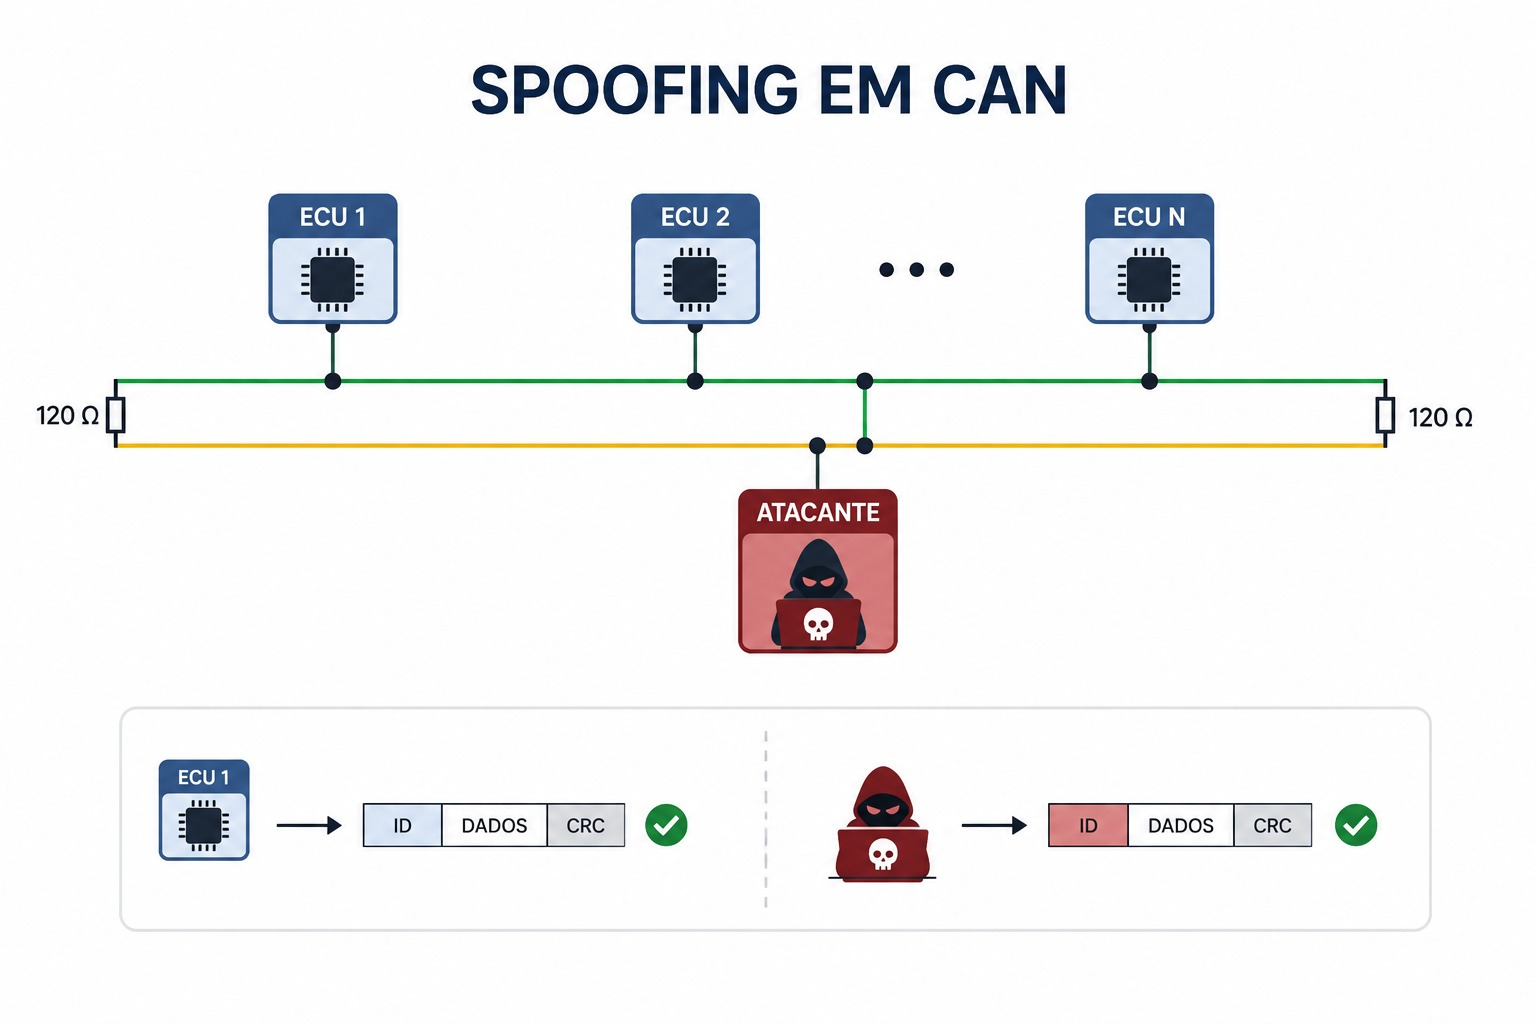
\includegraphics[width=1.0\textwidth]{images/spoofing.jpg}
    \caption{Ataque de \textit{Spoofing} em Barramento CAN}
    \label{fig:Spoofing}
\end{figure}

Um dos principais métodos de invasão nesse contexto é o ataque de \textit{spoofing}, no qual um dispositivo malicioso injeta quadros CAN utilizando identificadores válidos. Como o identificador no protocolo CAN representa o tipo ou prioridade da mensagem, e não a identidade do emissor, um atacante pode transmitir mensagens com o mesmo ID de uma ECU legítima, fazendo com que os demais nós aceitem essas mensagens como autênticas. Esse tipo de ataque permite a execução de comandos não autorizados e é considerado altamente relevante em cenários veiculares \cite{jo2021survey}.

Na prática, o ataque de \textit{spoofing} explora diretamente a ausência de autenticação no protocolo CAN. Como não existe um mecanismo capaz de verificar a origem legítima das mensagens transmitidas, qualquer nó conectado ao barramento pode enviar quadros válidos, desde que respeite a estrutura do protocolo \cite{cho2016fingerprinting}. Dessa forma, um invasor pode assumir logicamente o comportamento de uma ECU legítima sem necessariamente comprometer fisicamente o dispositivo original.

Esse tipo de ataque pode afetar diferentes sistemas do veículo, dependendo dos identificadores utilizados pelo atacante. Estudos demonstram que mensagens relacionadas ao controle do motor, direção, frenagem e painel de instrumentos podem ser falsificadas com relativa facilidade em ambientes experimentais \cite{nappi2020survey}. Como consequência, o \textit{spoofing} representa uma ameaça significativa à integridade funcional dos sistemas embarcados, especialmente em veículos modernos altamente interconectados \cite{sagstetter2013security}.

Além disso, ataques de \textit{spoofing} podem ser utilizados como etapa inicial para ataques mais complexos. Um agente malicioso pode utilizar mensagens falsificadas para induzir estados incorretos nas ECUs, mascarar informações legítimas ou provocar respostas inesperadas em outros módulos eletrônicos do veículo \cite{song2020vehicle}. Esse comportamento evidencia como a ausência de mecanismos de autenticação no CAN amplia a superfície de ataque do sistema \cite{girdhar2023cybersecurity}.

\subsection{Ataque de \textit{Replay}}

\begin{figure}[htbp]
    \centering
    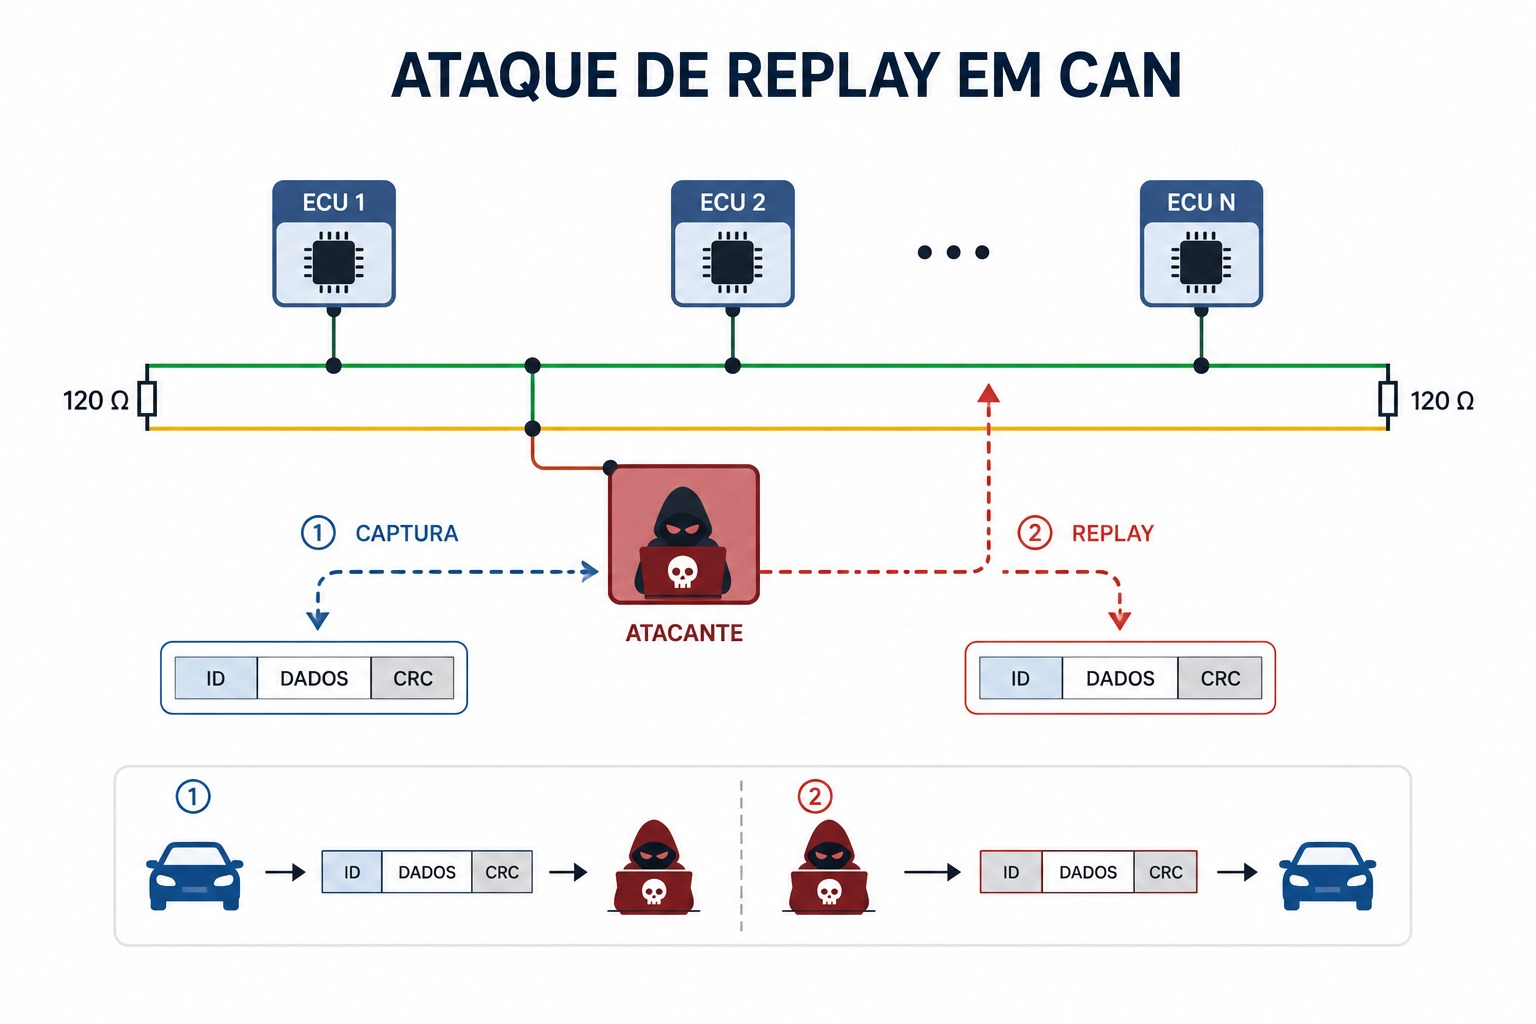
\includegraphics[width=1.0\textwidth]{images/replay.jpg}
    \caption{Ataque de \textit{Replay} em Barramento CAN}
    \label{fig:Replay}
\end{figure}

Outro método relevante é o ataque de \textit{replay}, que consiste na captura de quadros CAN válidos e sua retransmissão posterior. Esse ataque é viabilizado pela ausência de mecanismos como \textit{timestamps}, \textit{nonces} ou contadores de sequência no protocolo CAN, o que impede a verificação da atualidade das mensagens \cite{murvay2014source}. Como consequência, mensagens antigas podem ser aceitas como válidas, permitindo a repetição de comandos previamente executados \cite{bernardini2017security}.

Diferentemente do ataque de \textit{spoofing}, no qual o atacante precisa gerar novas mensagens, o ataque de \textit{replay} utiliza quadros legítimos previamente capturados no barramento. Isso reduz a necessidade de conhecimento aprofundado sobre o funcionamento interno das ECUs ou sobre o significado específico dos dados transmitidos \cite{studnia2018language}. Basta registrar uma sequência válida de mensagens e retransmiti-la posteriormente para reproduzir determinado comportamento do sistema.

Em redes CAN, esse tipo de ataque pode ser particularmente perigoso devido à natureza determinística da comunicação veicular. Como muitas mensagens são transmitidas periodicamente e possuem formatos previsíveis, torna-se relativamente simples capturar padrões de tráfego e reproduzi-los em momentos estratégicos \cite{van2011canauth}. Dessa forma, comandos válidos podem ser repetidos fora de contexto, comprometendo o funcionamento correto do veículo.

A ausência de mecanismos de verificação temporal no protocolo CAN também dificulta a identificação desse tipo de ataque. Como os quadros retransmitidos preservam identificadores e conteúdos válidos, os demais nós da rede tendem a aceitá-los como legítimos \cite{fernandez2023cybersecurity}. Em consequência, mecanismos criptográficos voltados apenas para confidencialidade ou integridade podem não ser suficientes para impedir ataques de \textit{replay}, sendo necessária a utilização de elementos adicionais de sincronização e validação temporal \cite{noureldeen2017replay}.

\subsection{Injeção de Mensagens}

\begin{figure}[htbp]
    \centering
    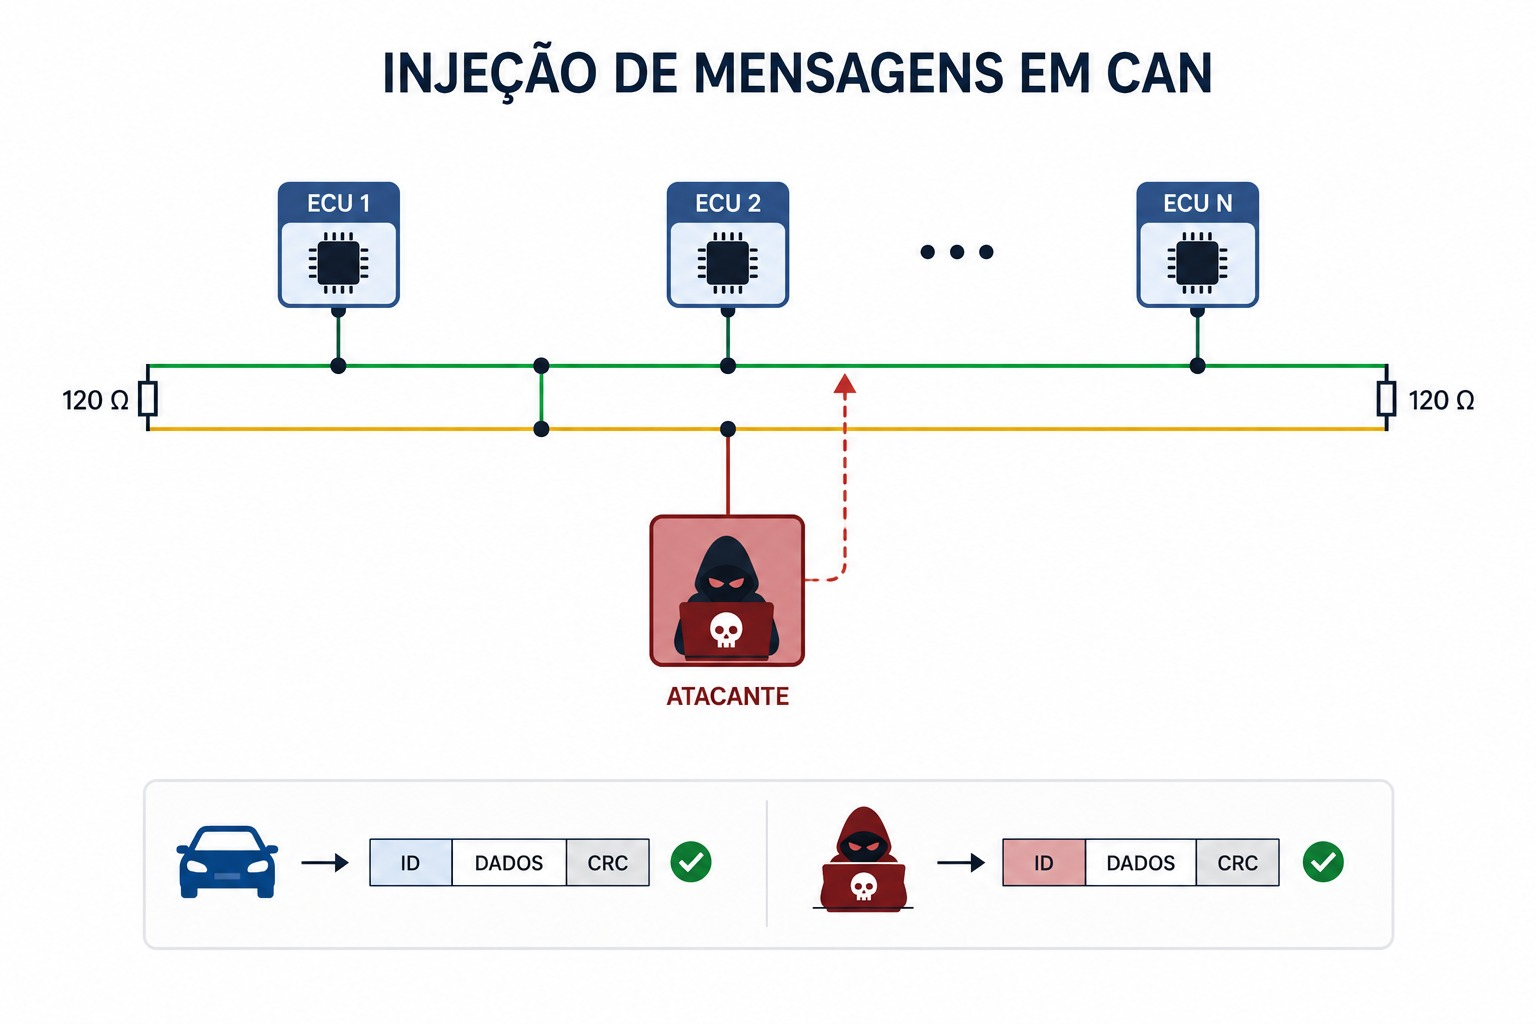
\includegraphics[width=1.0\textwidth]{images/injecao.jpg}
    \caption{Ataque de Injeção de Mensagens em Barramento CAN}
    \label{fig:Injecao}
\end{figure}

Além disso, destaca-se o ataque de injeção de mensagens, no qual um agente malicioso insere quadros arbitrários no barramento CAN. Esse tipo de ataque pode ser realizado a partir de acesso físico ao barramento, por exemplo, via porta OBD-II, ou por meio de interfaces externas comprometidas, como sistemas de \textit{infotainment} ou módulos de comunicação. A injeção de mensagens pode alterar diretamente o comportamento de sistemas críticos, dependendo dos identificadores utilizados \cite{dupont2019survey}.

Esse método de invasão é considerado um dos mais versáteis em redes CAN, pois permite que o atacante envie comandos específicos de acordo com seu objetivo \cite{aliwa2021cyberattacks}. Em cenários experimentais, pesquisadores demonstraram a possibilidade de controlar funções do veículo por meio da inserção de mensagens arbitrárias, incluindo alterações em indicadores do painel, acionamento de sistemas auxiliares e interferência em componentes relacionados à condução \cite{checkoway2011comprehensive}.

A eficiência desse tipo de ataque está diretamente relacionada ao conhecimento da estrutura das mensagens utilizadas pelo veículo. Embora o protocolo CAN defina apenas o formato geral dos quadros, o significado dos identificadores e dos dados transmitidos varia conforme o fabricante e o modelo do automóvel \cite{foster2015fast}. Assim, invasores frequentemente realizam engenharia reversa do tráfego CAN para identificar quais mensagens estão associadas a determinadas funções do sistema \cite{choi2021enhanced}.

Outro aspecto relevante é que a injeção de mensagens pode ocorrer tanto de forma isolada quanto em conjunto com outros ataques. Um invasor pode, por exemplo, utilizar técnicas de \textit{sniffing} para capturar o tráfego da rede, identificar padrões de comunicação e posteriormente injetar mensagens manipuladas no barramento. Essa combinação de técnicas amplia significativamente o potencial de comprometimento da rede veicular \cite{aliwa2021cyberattacks}.

\subsection{Negação de Serviço (\textit{Denial of Service -- DoS})}

\begin{figure}[htbp]
    \centering
    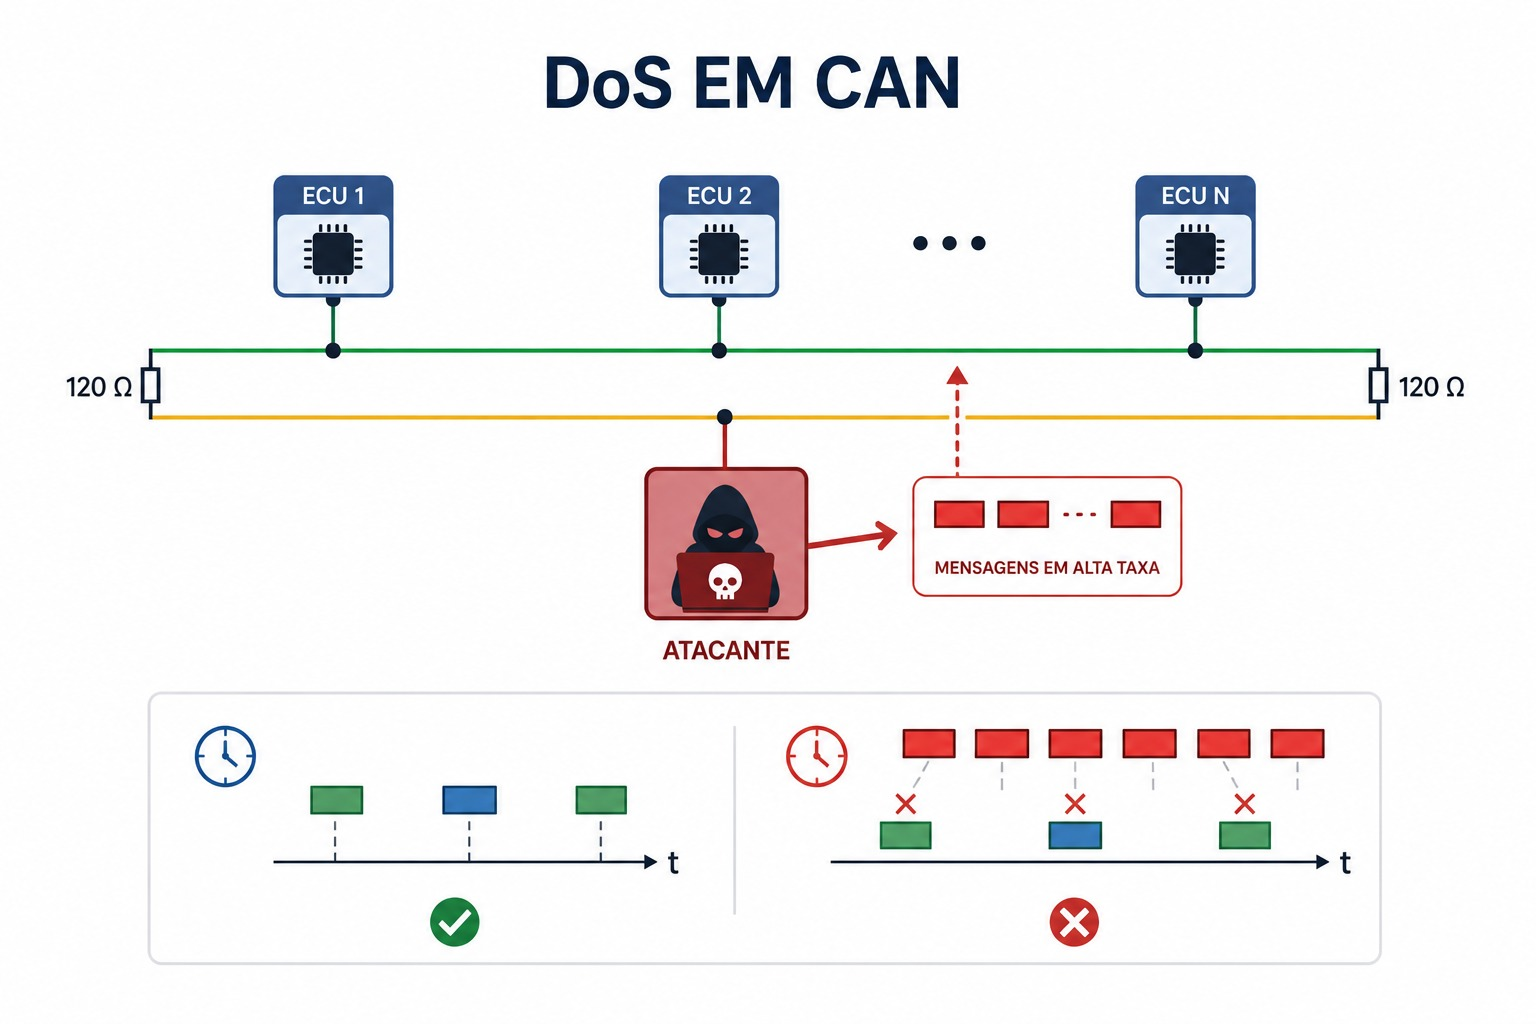
\includegraphics[width=1.0\textwidth]{images/dos.jpg}
    \caption{Ataque de Negação de Serviço em Barramento CAN}
    \label{fig:DoS}
\end{figure}

Outro vetor de ataque relevante é a negação de serviço (\textit{Denial of Service – DoS}), que explora o mecanismo de arbitragem bit a bit do protocolo CAN. Nesse processo, mensagens com identificadores de maior prioridade dominam o barramento, pois sobrescrevem bits recessivos durante a arbitragem. Um dispositivo malicioso pode explorar essa característica transmitindo continuamente mensagens de alta prioridade, causando \textit{starvation} de mensagens de menor prioridade e comprometendo a comunicação do sistema \cite{olivier2019hashing}.

O funcionamento do protocolo CAN depende da transmissão ordenada das mensagens no barramento compartilhado. Para evitar colisões destrutivas, o protocolo utiliza um mecanismo de arbitragem baseado nos identificadores das mensagens, no qual quadros com menor valor numérico possuem maior prioridade \cite{shi2022can}. Embora esse mecanismo seja eficiente para aplicações de tempo real, ele também cria uma vulnerabilidade explorável por agentes maliciosos \cite{lokman2019intrusion}.

Em um ataque de negação de serviço, o invasor transmite continuamente mensagens prioritárias, monopolizando o barramento e reduzindo drasticamente o espaço disponível para a comunicação das demais ECUs \cite{aliwa2021cyberattacks}. Como consequência, mensagens legítimas podem sofrer atrasos excessivos ou até deixar de ser transmitidas, comprometendo funções críticas do veículo \cite{li2010embedded}.

Dependendo da intensidade do ataque, o sistema pode apresentar degradação parcial ou falha completa de comunicação entre módulos eletrônicos. Em ambientes automotivos, esse comportamento é especialmente crítico devido à dependência de comunicação contínua entre ECUs responsáveis por funções relacionadas à segurança operacional \cite{dobaj2021cybersecurity}. Além disso, ataques de DoS apresentam difícil mitigação apenas com mecanismos criptográficos, pois exploram características estruturais do protocolo de acesso ao meio, e não necessariamente a falsificação do conteúdo das mensagens \cite{palanca2017stealth}.

\section{Avaliação de Desempenho de Algoritmos Criptográficos}

\begin{figure}[htbp]
    \centering
    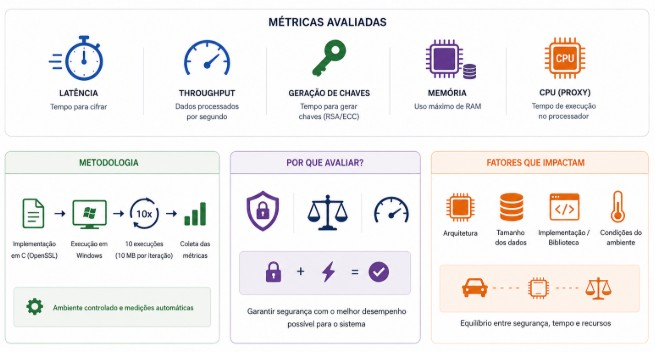
\includegraphics[width=1.0\textwidth]{images/medidas.jpg}
    \caption{Avaliação do Desempenho dos Algoritmos Criptográficos}
    \label{fig:desempenho}
\end{figure}

A avaliação de desempenho de algoritmos criptográficos é essencial para sua aplicação em sistemas embarcados, especialmente em contextos com restrições de tempo real e recursos computacionais limitados. Nesses ambientes, o uso de criptografia introduz \textit{overhead} computacional que pode impactar diretamente o comportamento do sistema, tornando necessária a mensuração objetiva de seu custo \cite{perrig2001spins}.

A análise de desempenho é realizada por meio da mensuração de métricas específicas, considerando como unidade de operação a cifragem de dados. Essa escolha se deve ao fato de que o objetivo é avaliar o impacto direto da aplicação de algoritmos criptográficos na proteção de mensagens, sendo a operação de cifragem representativa do custo computacional envolvido na transmissão de dados protegidos \cite{gura2004comparing}.

A latência de criptografia é definida como o tempo necessário para executar a operação de cifragem de um conjunto de dados. Essa métrica é expressa em segundo(s) e foi medida utilizando funções de temporização de alta resolução, considerando o tempo total de execução dividido pelo número de iterações realizadas \cite{stankovic1996real}. Formalmente, a latência média pode ser definida como:

\[
\text{Latência média} = \frac{T_{total}}{N}
\]

em que $T_{total}$ representa o tempo total de execução e $N$ o número de iterações.

O \textit{throughput} representa a quantidade de dados processados por unidade de tempo, sendo expresso em megabytes por segundo (MB/s). Essa métrica foi calculada a partir da relação entre o volume total de dados processados e o tempo de execução, conforme \cite{tanenbaum1981network}:

\[
\textit{Throughput} = \frac{D \times N}{T_{total}}
\]

em que $D$ representa o tamanho dos dados processados em cada iteração, como exemplo, considerando um processamento de 1 MB por iteração, com 10 execuções em um tempo total de 2 segundos, o \textit{throughput} obtido seria de 5 MB/s.

A escolha do volume de dados de 1 MB por iteração não representa diretamente o tamanho das mensagens do barramento CAN, que são significativamente menores, mas foi adotada com o objetivo de reduzir o efeito de sobrecarga de chamadas de função e aumentar a estabilidade das medições. Essa abordagem é comum em avaliações de desempenho, pois permite obter resultados mais consistentes ao amortizar custos fixos de execução \cite{singh2024advanced}.

Além disso, foi avaliado o tempo de geração de chaves, particularmente relevante para algoritmos assimétricos como RSA e ECC. Essa métrica corresponde ao tempo necessário para a criação de pares de chaves criptográficas, sendo expressa em segundos e medida diretamente a partir da execução das funções de geração de chaves. Estudos indicam que algoritmos assimétricos apresentam custo significativamente superior em relação aos simétricos, especialmente em operações de geração de chaves \cite{gaubatz2004public}.

O consumo de memória foi mensurado com base no uso máximo de memória RAM durante a execução do programa, expresso em kilobytes (KB), utilizando chamadas de sistema específicas. Essa métrica permite avaliar o impacto dos algoritmos em ambientes com restrições de memória, sendo particularmente relevante em dispositivos embarcados \cite{silva2016case}.

No que se refere ao uso de CPU, a análise foi conduzida de forma indireta, utilizando o tempo de execução como métrica \textit{proxy}. Em ambiente controlado, sem interferência significativa de outros processos, o tempo de execução está diretamente relacionado à carga computacional imposta pelo algoritmo, permitindo inferir seu custo de processamento \cite{pham2017development}.

A coleta das métricas foi realizada ao longo de múltiplas execuções, sendo adotado um número fixo de iterações para reduzir variações e aumentar a confiabilidade dos resultados. Embora o número inicial de 10 iterações permita uma avaliação preliminar, esse valor pode ser ampliado para melhorar a precisão estatística dos resultados, reduzindo o impacto de variações ocasionais no tempo de execução \cite{georges2007statistically}.

O ambiente experimental foi definido de forma controlada, utilizando linguagem C e a biblioteca OpenSSL para implementação dos algoritmos criptográficos. A execução foi realizada em um sistema computacional com arquitetura baseada em CPU de uso geral, sob sistema operacional do tipo \textit{Windows}, em ambiente isolado, sem a execução de aplicações concorrentes relevantes, garantindo maior consistência nas medições \cite{dierks2008transport}.

Cabe destacar que, embora o conceito de \textit{handshake} seja relevante em protocolos criptográficos, especialmente em contextos de comunicação segura, ele não é diretamente aplicável ao escopo deste trabalho, uma vez que a análise se concentra no desempenho isolado dos algoritmos. Dessa forma, optou-se por não incluir essa métrica, focando exclusivamente em operações mensuráveis no contexto experimental definido.

Dessa forma, a metodologia adotada permite avaliar de forma objetiva o desempenho dos algoritmos AES-128, ChaCha20, RSA e ECC, considerando métricas diretamente relacionadas ao seu custo computacional. Essa abordagem possibilita a análise dos \textit{trade-offs} entre segurança e eficiência, fornecendo subsídios técnicos para sua aplicação em sistemas embarcados e comunicação em barramentos CAN \cite{roman2011securing}.a adotada permite avaliar de forma objetiva o desempenho dos algoritmos AES-128, ChaCha20, RSA e ECC, considerando métricas diretamente relacionadas ao seu custo computacional. Essa abordagem possibilita a análise dos \textit{trade-offs} entre segurança e eficiência, fornecendo subsídios técnicos para sua aplicação em sistemas embarcados e comunicação em barramentos CAN.

\section{Uso da Biblioteca OpenSSL}

\begin{figure}[htbp]
    \centering
    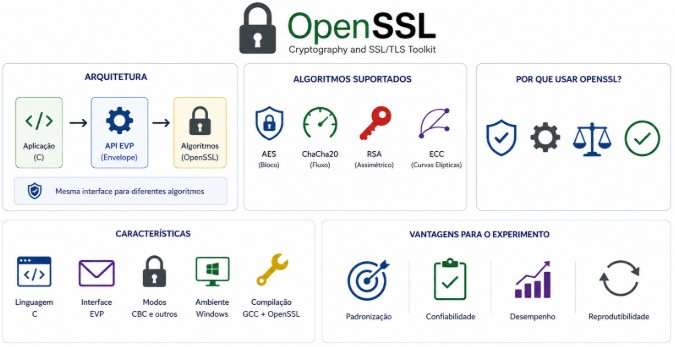
\includegraphics[width=1.0\textwidth]{images/OpenSSL.jpg}
    \caption{Entendimento sobre a Biblioteca OpenSSL}
    \label{fig:openssl}
\end{figure}

A biblioteca OpenSSL pode ser utilizada como base para a implementação dos algoritmos criptográficos, devido à necessidade de utilizar implementações consolidadas e otimizadas, capazes de representar de forma fiel o comportamento desses algoritmos em aplicações práticas. Diferentemente de implementações simplificadas ou acadêmicas, o uso de uma biblioteca consolidada reduz a influência de erros de implementação e garante maior validade experimental na análise de desempenho \cite{ferguson2011cryptography}.

A OpenSSL disponibiliza implementações eficientes de algoritmos criptográficos amplamente utilizados, como AES, ChaCha20, RSA e ECC, permitindo que a avaliação conduzida neste trabalho seja baseada em implementações reais, e não em versões experimentais. Esse aspecto é fundamental, pois o desempenho de algoritmos criptográficos pode variar significativamente conforme a qualidade da implementação, impactando diretamente os resultados obtidos \cite{openssl2023}.

Um ponto central na utilização da OpenSSL é o uso da API EVP (\textit{Envelope}), que fornece uma interface padronizada para a execução de diferentes algoritmos criptográficos. Essa abstração permite que algoritmos distintos sejam utilizados sob uma mesma estrutura de chamadas, eliminando variações decorrentes da forma de implementação. Dessa forma, a utilização da API EVP possibilita uma comparação mais justa entre os algoritmos avaliados, garantindo que as diferenças observadas nos resultados estejam relacionadas ao comportamento intrínseco de cada algoritmo, e não a diferenças na forma de implementação \cite{viega2002network}.

Como exemplo, o trecho a seguir apresenta uma forma simplificada de utilização da API EVP para cifrar dados com o algoritmo ChaCha20. O objetivo do exemplo não é representar a implementação completa do experimento, mas ilustrar como a biblioteca OpenSSL permite inicializar um contexto criptográfico, definir chave e \textit{nonce}, processar os dados de entrada e obter uma saída cifrada por meio de uma interface padronizada \cite{openssl2023}.

\begin{lstlisting}[language=C, caption={Exemplo simplificado de cifragem com ChaCha20 utilizando OpenSSL}, label={lst:chacha20_openssl}]
#include <openssl/evp.h>
#include <string.h>

int main() {
unsigned char chave[32] = {0};
unsigned char nonce[16] = {0};

unsigned char entrada[8] = {
    0x64, 0x32, 0x00, 0x01,
    0x15, 0x08, 0x00, 0xFF
};

unsigned char saida[8];
int tamanho_saida = 0;

EVP_CIPHER_CTX *ctx = EVP_CIPHER_CTX_new();

EVP_EncryptInit_ex(ctx, EVP_chacha20(), NULL, chave, nonce);

EVP_EncryptUpdate(
    ctx,
    saida,
    &tamanho_saida,
    entrada,
    sizeof(entrada)
);

EVP_CIPHER_CTX_free(ctx);

return 0;

}
\end{lstlisting}

No exemplo, o vetor \texttt{entrada} representa uma carga útil hipotética de 8 bytes, compatível com o tamanho máximo do campo de dados de uma mensagem CAN clássica. Após a execução da função \texttt{EVP\_EncryptUpdate}, os bytes cifrados são armazenados no vetor \texttt{saida}. Esse tipo de estrutura é semelhante ao funcionamento adotado no experimento, no qual os dados extraídos dos \textit{datasets} CAN são processados pelos algoritmos criptográficos avaliados \cite{openssl2023,viega2002network}.

Além disso, a padronização proporcionada pela API EVP contribui para a consistência metodológica do experimento, uma vez que assegura que todos os algoritmos sejam avaliados sob condições equivalentes de execução. Esse fator é particularmente relevante em análises comparativas, nas quais a ausência de padronização pode comprometer a validade dos resultados \cite{georges2007statistically}.

Dessa forma, a utilização da biblioteca OpenSSL não se limita à viabilização da implementação dos algoritmos, mas constitui um elemento fundamental para a confiabilidade da análise experimental, ao garantir que os resultados obtidos reflitam o desempenho de implementações reais, avaliadas de forma consistente e comparável \cite{krovetz2011software}.

\section{Benchmarking e Métricas de Avaliação}

\begin{figure}[htbp]
    \centering
    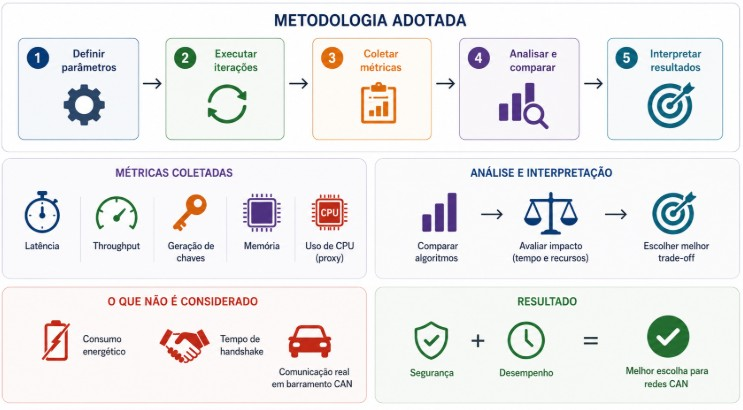
\includegraphics[width=1.0\textwidth]{images/benchmark.jpg}
    \caption{Benchmark e as Métricas para serem Avaliadas}
    \label{fig:benchmark}
\end{figure}

A avaliação de desempenho de algoritmos criptográficos é realizada por meio de técnicas de \textit{benchmarking}, com o objetivo de comparar o custo computacional associado à aplicação de diferentes algoritmos na proteção de dados. A adoção dessa abordagem está diretamente relacionada à necessidade de analisar, de forma objetiva, o impacto da criptografia em sistemas embarcados, especialmente no contexto de comunicação em barramentos CAN, nos quais restrições de tempo e recursos são fatores críticos \cite{hennessy2011computer}.

Diferentemente de abordagens genéricas de avaliação, este trabalho concentra-se em métricas diretamente relacionadas ao custo computacional das operações criptográficas, permitindo analisar seu impacto prático na transmissão de dados. Nesse sentido, foram selecionadas as métricas de latência, \textit{throughput}, tempo de geração de chaves e consumo de recursos computacionais, por representarem fatores determinantes na viabilidade da aplicação de criptografia nesse contexto \cite{paar2010understanding}.

A latência foi escolhida como métrica central por representar o tempo necessário para a execução da operação de cifragem. O aumento desse tempo impacta diretamente o processamento das mensagens, sendo um fator relevante em sistemas que dependem de respostas em intervalos restritos \cite{pinho2001timing}.

O \textit{throughput}, por sua vez, complementa a análise ao indicar a quantidade de dados processados por unidade de tempo, sendo geralmente expresso em megabytes por segundo (MB/s). De modo geral, há uma tendência de que algoritmos com menor tempo de execução apresentem maior capacidade de processamento. No entanto, essa relação não é estritamente linear, podendo ser influenciada por fatores como \textit{overhead} de implementação, organização interna do algoritmo e características da execução, o que torna necessária a análise conjunta dessas métricas para uma avaliação mais precisa \cite{mckeen2013innovative}.

O tempo de geração de chaves foi incluído na análise por ser uma métrica relevante para algoritmos assimétricos, como RSA e ECC, cujas operações apresentam custo computacional significativamente superior em comparação com algoritmos simétricos. Embora essa operação não ocorra com a mesma frequência que a cifragem de dados, seu impacto pode ser relevante em processos de inicialização ou estabelecimento de comunicação segura \cite{goyal2022energy}.

O consumo de recursos computacionais, incluindo uso de CPU e memória, também foi considerado, uma vez que limitações nesses recursos podem afetar a execução de outras tarefas no sistema. Algoritmos que demandam maior uso de memória ou processamento podem se tornar inviáveis dependendo do ambiente de aplicação \cite{sass2010embedded}.

Por outro lado, métricas como consumo energético e tempo de \textit{handshake} não foram incluídas neste trabalho. O consumo energético, embora relevante em determinados cenários, não foi considerado devido à ausência de instrumentação específica para medição precisa no ambiente experimental adotado. Já o tempo de \textit{handshake} está associado a protocolos de comunicação segura, não sendo diretamente aplicável ao escopo deste estudo, que se concentra na análise isolada do desempenho dos algoritmos criptográficos \cite{rescorla2001ssl}.

Além disso, a escolha do tamanho dos dados processados influencia diretamente as métricas analisadas. Neste trabalho, será adotado um volume de dados superior ao tamanho típico de mensagens CAN, com o objetivo de reduzir o impacto de sobrecargas associadas à execução de funções e obter medições mais estáveis. Essa abordagem é consistente com práticas de avaliação de desempenho que buscam minimizar interferências externas e aumentar a confiabilidade dos resultados \cite{mytkowicz2009producing}.

A utilização de \textit{benchmarking} para avaliação de algoritmos criptográficos, no contexto deste trabalho, tem como objetivo mensurar o custo computacional associado à proteção de dados e relacioná-lo ao impacto na transmissão de mensagens em barramentos CAN. Como o ambiente experimental não envolve a comunicação real em um barramento físico, os dados obtidos representam exclusivamente o desempenho de processamento dos algoritmos, sendo necessária a construção de um modelo que permita interpretar esses resultados no contexto da comunicação CAN \cite{jain2010art,hennessy2011computer}.

Conforme discutido anteriormente, a latência total de uma mensagem protegida resulta da combinação entre o tempo de processamento criptográfico e a latência de comunicação no barramento CAN. No presente trabalho, apenas $Lat_{proc}$ é mensurado diretamente por meio do benchmark, sendo $Lat_{comm}$ dependente das características do barramento CAN, como taxa de transmissão, carga e mecanismos de arbitragem \cite{specification1991bosch}.

A latência de comunicação em redes CAN apresenta variação conforme a taxa de transmissão configurada. Em um barramento operando a 125 kbps, a transmissão de um quadro pode atingir aproximadamente 1 ms, enquanto em 500 kbps esse valor reduz-se para a ordem de 200 a 300 $\mu$s, dependendo do tamanho do quadro e das condições de arbitragem \cite{navet2017automotive}. Esses valores fornecem uma base quantitativa para avaliar a relevância do custo criptográfico no contexto de sistemas de tempo real.

A latência de processamento $Lat_{proc}$ é obtida experimentalmente a partir do tempo total de execução $T_{proc}$ (em segundos) para o processamento de um volume de dados $D$ (em bytes). A partir desses valores, define-se o custo médio de processamento por byte:

\begin{equation}
C_{byte} = \frac{T_{proc}}{D} \quad [s/byte]
\end{equation}

Esse parâmetro permite projetar o impacto da criptografia sobre mensagens CAN. Considerando o padrão CAN clássico, no qual o campo de dados possui até 8 bytes, a latência adicional por mensagem pode ser estimada por:

\begin{equation}
Lat_{msg} \approx C_{byte} \times 8
\end{equation}

Essa aproximação assume proporcionalidade entre o volume de dados processado e o tempo de execução, sendo tratada como hipótese de modelagem \cite{montgomery2017design}. A validade dessa hipótese será investigada experimentalmente por meio da análise da relação entre diferentes tamanhos de entrada e o tempo de execução, permitindo verificar a adequação da aproximação linear para os algoritmos analisados.

Para validar o modelo proposto, será realizada a comparação entre o tempo estimado e o tempo medido experimentalmente. Define-se o erro relativo como:

\begin{equation}
Erro = \frac{|T_{real} - T_{estimado}|}{T_{real}}
\end{equation}

em que $T_{real}$ corresponde ao tempo medido e $T_{estimado}$ ao valor obtido a partir do modelo. A interpretação desse erro será realizada de forma comparativa, considerando a variabilidade das medições em ambiente controlado, conforme discutido em metodologias de avaliação de desempenho \cite{jain2010art}. Dessa forma, não se estabelece um limite fixo universal, mas sim uma análise baseada na consistência dos resultados obtidos.

Como exemplo de aplicação do modelo, considere um experimento no qual $T_{proc} = 2s$ para o processamento de $D = 10MB$. Nesse caso, tem-se:

\begin{equation}
C_{byte} = \frac{2}{10 \times 1024 \times 1024} \approx 1{,}9 \times 10^{-7} \; s/byte
\end{equation}

A partir disso, a latência estimada para uma mensagem CAN de 8 bytes é:

\begin{equation}
Lat_{msg} \approx 1{,}9 \times 10^{-7} \times 8 \approx 1{,}5 \, \mu s
\end{equation}

Considerando uma taxa de 1000 mensagens por segundo, o impacto acumulado será:

\begin{equation}
Lat_{acum} = 1000 \times 1{,}5 \, \mu s = 1{,}5 \, ms
\end{equation}

Esse valor permite comparar diretamente o custo da criptografia com a latência do barramento, evidenciando que, dependendo do algoritmo utilizado, o impacto pode se tornar relevante em cenários de alta frequência de mensagens \cite{burns2001real}.

Deve-se destacar que algoritmos criptográficos apresentam comportamentos distintos quanto à relação entre volume de dados e tempo de execução. Algoritmos simétricos, como AES e ChaCha20, tendem a apresentar comportamento aproximadamente linear para volumes maiores de dados, sendo adequados à modelagem por custo por byte \cite{bernstein2008chacha}. Por outro lado, algoritmos assimétricos, como RSA e ECC, possuem custo dominado por operações matemáticas discretas, sendo mais adequados para análise baseada em tempo de geração de chaves e operações pontuais, e não diretamente pela métrica de custo por byte \cite{gura2004comparing}.

Adicionalmente, algoritmos baseados em blocos, como o AES, operam sobre unidades fixas de dados (tipicamente 16 bytes), o que pode introduzir efeitos de \textit{padding} em mensagens menores, como no caso do CAN clássico \cite{daemen2002design}. Essa característica constitui uma limitação do modelo adotado.

O impacto acumulado da criptografia pode ser estimado considerando uma taxa de $N$ mensagens por segundo:

\begin{equation}
Lat_{acum} = N \times Lat_{msg}
\end{equation}

Esse modelo assume acúmulo linear do atraso, com independência entre mensagens e ausência de paralelismo, sendo adequado para fins comparativos em ambiente controlado \cite{morgan1984discrete}.

A escolha de volumes de dados maiores no \textit{benchmark} tem como objetivo reduzir a influência de \textit{overheads} fixos, como inicialização de contexto e chamadas de função, permitindo estimativas mais estáveis do custo computacional dos algoritmos \cite{hennessy2011computer}.

A partir do modelo proposto, a comparação entre algoritmos criptográficos é realizada com base em critérios quantitativos. Define-se como critério principal o menor impacto na latência por mensagem ($Lat_{msg}$) e como critério complementar o menor impacto acumulado ($Lat_{acum}$). Para algoritmos assimétricos, considera-se adicionalmente o custo de geração de chaves \cite{goyal2022energy}.

Cabe destacar que, embora o desempenho seja o foco da análise, os algoritmos avaliados são assumidos como seguros quando utilizados com parâmetros recomendados, sendo a segurança tratada como requisito de base \cite{ferguson2011cryptography}.

A hipótese de pesquisa estabelece que algoritmos simétricos apresentam menor custo computacional e, consequentemente, menor impacto na latência de mensagens. No entanto, a principal contribuição deste trabalho consiste na quantificação desse impacto no contexto de barramentos CAN, por meio da aplicação de um modelo que relaciona resultados de \textit{benchmark} ao comportamento do sistema \cite{henia2005system}.


\section{Síntese dos Trabalhos Relacionados e Lacuna de Pesquisa}

Os estudos apresentados nesta fundamentação abordam diferentes aspectos da utilização de criptografia em sistemas embarcados e redes automotivas. Pesquisas relacionadas à segurança do barramento CAN destacam vulnerabilidades associadas à ausência de mecanismos nativos de criptografia e autenticação, evidenciando a necessidade de soluções de proteção compatíveis com as características da comunicação automotiva \cite{bozdal2020evaluation,lotto2024survey}.

No contexto do desempenho criptográfico, estudos demonstram a importância das características da plataforma computacional para a eficiência dos mecanismos utilizados. A utilização de instruções específicas de hardware pode acelerar a execução do AES, enquanto as características de implementação das cifras de fluxo também influenciam seu desempenho em diferentes ambientes computacionais \cite{gueron2010intel,manifavas2016survey}. Além disso, avaliações experimentais de algoritmos criptográficos leves em redes IoT sem fio reforçam a relevância da mensuração de custos computacionais em dispositivos com recursos limitados \cite{blanc2022benchmarking}.

Em relação à criptografia aplicada à segurança veicular, a literatura também apresenta abordagens voltadas à utilização de mecanismos criptográficos em arquiteturas de proteção automotiva, considerando requisitos de segurança e limitações dos sistemas embarcados \cite{mundhenk2017security}.

A análise conjunta dessas contribuições evidencia a importância de considerar as características da plataforma computacional, as operações executadas e as propriedades de segurança de cada mecanismo. Entretanto, a avaliação de desempenho exige distinguir os custos da cifragem simétrica por mensagem daqueles associados às operações assimétricas e híbridas, evitando comparações que desconsiderem suas diferentes funções. Também é necessário separar a latência de processamento criptográfico da latência total de transmissão pelo barramento CAN.

Nesse contexto, o presente trabalho propõe uma avaliação experimental dos mecanismos AES-128-CTR, ChaCha20, RSA-2048-OAEP e ECIES-P256, utilizando um computador com OpenSSL e uma plataforma embarcada ESP32 com mbedTLS. A contribuição consiste em caracterizar os custos computacionais observados nesses ambientes, considerando principalmente a latência de processamento, as diferenças funcionais entre os mecanismos e as limitações de cada configuração experimental. A pesquisa não pretende estabelecer superioridade universal entre os mecanismos nem avaliar a segurança de um protocolo CAN completo.
